% Options for packages loaded elsewhere
\PassOptionsToPackage{unicode}{hyperref}
\PassOptionsToPackage{hyphens}{url}
\documentclass[
]{article}
\usepackage{xcolor}
\usepackage[margin=1in]{geometry}
\usepackage{amsmath,amssymb}
\setcounter{secnumdepth}{5}
\usepackage{iftex}
\ifPDFTeX
  \usepackage[T1]{fontenc}
  \usepackage[utf8]{inputenc}
  \usepackage{textcomp} % provide euro and other symbols
\else % if luatex or xetex
  \usepackage{unicode-math} % this also loads fontspec
  \defaultfontfeatures{Scale=MatchLowercase}
  \defaultfontfeatures[\rmfamily]{Ligatures=TeX,Scale=1}
\fi
\usepackage{lmodern}
\ifPDFTeX\else
  % xetex/luatex font selection
\fi
% Use upquote if available, for straight quotes in verbatim environments
\IfFileExists{upquote.sty}{\usepackage{upquote}}{}
\IfFileExists{microtype.sty}{% use microtype if available
  \usepackage[]{microtype}
  \UseMicrotypeSet[protrusion]{basicmath} % disable protrusion for tt fonts
}{}
\makeatletter
\@ifundefined{KOMAClassName}{% if non-KOMA class
  \IfFileExists{parskip.sty}{%
    \usepackage{parskip}
  }{% else
    \setlength{\parindent}{0pt}
    \setlength{\parskip}{6pt plus 2pt minus 1pt}}
}{% if KOMA class
  \KOMAoptions{parskip=half}}
\makeatother
\usepackage{longtable,booktabs,array}
\usepackage{calc} % for calculating minipage widths
% Correct order of tables after \paragraph or \subparagraph
\usepackage{etoolbox}
\makeatletter
\patchcmd\longtable{\par}{\if@noskipsec\mbox{}\fi\par}{}{}
\makeatother
% Allow footnotes in longtable head/foot
\IfFileExists{footnotehyper.sty}{\usepackage{footnotehyper}}{\usepackage{footnote}}
\makesavenoteenv{longtable}
\usepackage{graphicx}
\makeatletter
\newsavebox\pandoc@box
\newcommand*\pandocbounded[1]{% scales image to fit in text height/width
  \sbox\pandoc@box{#1}%
  \Gscale@div\@tempa{\textheight}{\dimexpr\ht\pandoc@box+\dp\pandoc@box\relax}%
  \Gscale@div\@tempb{\linewidth}{\wd\pandoc@box}%
  \ifdim\@tempb\p@<\@tempa\p@\let\@tempa\@tempb\fi% select the smaller of both
  \ifdim\@tempa\p@<\p@\scalebox{\@tempa}{\usebox\pandoc@box}%
  \else\usebox{\pandoc@box}%
  \fi%
}
% Set default figure placement to htbp
\def\fps@figure{htbp}
\makeatother
% definitions for citeproc citations
\NewDocumentCommand\citeproctext{}{}
\NewDocumentCommand\citeproc{mm}{%
  \begingroup\def\citeproctext{#2}\cite{#1}\endgroup}
\makeatletter
 % allow citations to break across lines
 \let\@cite@ofmt\@firstofone
 % avoid brackets around text for \cite:
 \def\@biblabel#1{}
 \def\@cite#1#2{{#1\if@tempswa , #2\fi}}
\makeatother
\newlength{\cslhangindent}
\setlength{\cslhangindent}{1.5em}
\newlength{\csllabelwidth}
\setlength{\csllabelwidth}{3em}
\newenvironment{CSLReferences}[2] % #1 hanging-indent, #2 entry-spacing
 {\begin{list}{}{%
  \setlength{\itemindent}{0pt}
  \setlength{\leftmargin}{0pt}
  \setlength{\parsep}{0pt}
  % turn on hanging indent if param 1 is 1
  \ifodd #1
   \setlength{\leftmargin}{\cslhangindent}
   \setlength{\itemindent}{-1\cslhangindent}
  \fi
  % set entry spacing
  \setlength{\itemsep}{#2\baselineskip}}}
 {\end{list}}
\usepackage{calc}
\newcommand{\CSLBlock}[1]{\hfill\break\parbox[t]{\linewidth}{\strut\ignorespaces#1\strut}}
\newcommand{\CSLLeftMargin}[1]{\parbox[t]{\csllabelwidth}{\strut#1\strut}}
\newcommand{\CSLRightInline}[1]{\parbox[t]{\linewidth - \csllabelwidth}{\strut#1\strut}}
\newcommand{\CSLIndent}[1]{\hspace{\cslhangindent}#1}
\setlength{\emergencystretch}{3em} % prevent overfull lines
\providecommand{\tightlist}{%
  \setlength{\itemsep}{0pt}\setlength{\parskip}{0pt}}
\usepackage{multirow}
\usepackage{bookmark}
\IfFileExists{xurl.sty}{\usepackage{xurl}}{} % add URL line breaks if available
\urlstyle{same}
\hypersetup{
  pdftitle={Thesis - StrongHER Project: Exploring the Impact of Nutrition on Bone Health in Female Athletes},
  hidelinks,
  pdfcreator={LaTeX via pandoc}}

\title{Thesis - StrongHER Project: Exploring the Impact of Nutrition on Bone Health in Female Athletes}
\author{Principal Investigator: Katriona Ross\\
Co-Investigator(s):\\
Dr Fergus Guppy (Associate Professor)\\
Dr Hannah Lithgow (Assistant Professor)\\
Dr David King (Assistant Professor)}
\date{2024-12-11}

\begin{document}
\maketitle

{
\setcounter{tocdepth}{2}
\tableofcontents
}
\section{Introduction}\label{introduction}

\subsection{What is already known/reported on this topic?}\label{what-is-already-knownreported-on-this-topic}

\begin{enumerate}
\def\labelenumi{\arabic{enumi}.}
\item
  It is known that low energy availability (LEA) because of insufficient calorie intake or over training can lead to amenorrhea and bone health conditions such as low bone mineral density (BMD) or osteoporosis long term.
\item
  It is known that inadequate intake of essential nutrients such as calcium, vitamin D will significantly affect BMD.
\item
  It is known that both LEA and poor micronutrient intakes are common in female athletes who are at further increased risk if they are training indoors or live in norther latitudes.
\end{enumerate}

\subsection{What could this study add?}\label{what-could-this-study-add}

\begin{enumerate}
\def\labelenumi{\arabic{enumi}.}
\item
  Longitudinal data tracking changes in bone health, energy availability and nutrient intakes over time.
\item
  More high-quality research in female athletes, an understudied population.
\item
  Research across different sporting populations i.e.~indoor vs outdoor, impact vs non-impact.
\item
  Investigate the efficacy and use of BIA for early detection of LEA compared to currently used diagnostic criteria.
\item
  Could help identify potential future interventions for nutrition in female athletes for improved bone health and energy availability.
\end{enumerate}

\subsection{Potential for this study to affect practice, research or policy}\label{potential-for-this-study-to-affect-practice-research-or-policy}

The proposed study holds significant implications for advancing our understanding of energy availability (EA), micronutrient status and bone health in female athletes. By addressing these critical gaps in knowledge, the research aims to optimise both health and performance outcomes. The findings will not only contribute to academic knowledge but also provide practical insights for coaches, nutritionists, and practitioners working with female athletes.

\section{Background \& Rationale}\label{background-rationale}

Research shows a substantial under-representation of women with only 6-12\% of all studies utilising female-only participants (Cowley et al. 2021; Hutchins et al. 2021). Furthermore, only 10\% of the studies used elite or highly trained athletes (Smith et al. 2022). This underrepresentation of female athletes in sport science and sport medicine (SSSM) research may have significant implications on our understanding of the unique physiological factors impacting female athlete health and performance. Additionally, the methodological quality of studies conducted on female athletes has been compromised due to historical neglect and a lack of understanding of reproductive endocrinology. Traditionally, sport and exercise science data have primarily originated from studies involving male participants, resulting in a dearth of high-quality data applicable to female athletes (Elliott-Sale et al. 2021). Applying evidence developed based on male athlete research to female cohorts may be erroneous and with significant challenges (Emmonds, Heyward, and Jones 2019)

Therefore, one of the aims of this study is to produce high-quality female-specific data through a more comprehensive and tailored approach to research, ultimately contributing to a more robust understanding of the unique physiological considerations in female athletes.

\subsection{Overview of Bone Health in Female Athletes}\label{overview-of-bone-health-in-female-athletes}

Athletes, particularly female athletes are at increased risk of developing bone injuries and bone-related conditions, such as stress fractures, osteoporosis and osteopenia due to imbalance between training and recovery (Goolsby and Boniquit 2017). Bone health is multifactorial, adequate nutrition, sufficient mechanical stimulus, hormonal, genetic and environmental factors all playing a role in achieving and maintaining optimal bone health in athletes. The primary concern for athletes and support staff being the avoidance of injury as this will directly influence performance. In addition to affecting athletic performance, optimal bone health is essential for long-term well-being of female athletes as poor bone health can lead to more chronic conditions later in life.

At present, osteoporosis affects 1 in 3 women compared to 1 in 5 men. Additionally, the number of hip fractures in the UK due to osteoporosis has risen from 70,000 in 2006 to 100,000 in 2020, an increase of 44\% (Stevenson 2023). Consequently, there is both a significant economic burden and a clear impact on the quality of life of those affected. The heightened vulnerability of female athletes to bone injuries and related conditions underscores the crucial role of nutrition in fostering optimal bone health.

Stress fractures and bone stress injuries, resulting from overuse and increased mechanical loading are common in many sports (McBryde 1985), with these injuries being complex and not completely understood, current evidence suggests that dietary restraint, suboptimal vitamin D status (\textless30ng/ml) and menstrual dysfunction are risk factors for sustaining bone stress injuries (Barrack et al. 2014; Bishop et al. 2021; Neal et al. 2015). Vitamin D plays a crucial role in calcium absorption and bone metabolism making it a key nutrient for bone health.

**Explain here some context of why BMD is a useful marker of skeletal health would be useful

The interplay between diet and exercise training is also critical in better understanding the long-term bone health of retired athletes, with the avoidance of conditions such as osteopenia and osteoporosis crucial in maintaining a healthy lifespan in this population. This involves maximising peak bone mineral density (BMD), which relates to the strength of the internal bone tissue, in relation to microarchitecture and geometry and managing the rate of bone loss with increasing age (Bailey and Brooke-Wavell 2008). As ninety percent of peak bone mass is accrued by age 20 and then, after a period of stability BMD will begin to decline as women reach their late 30's. Men not only exhibit higher total BMD but are also less susceptible to age related bone loss than women (Santos, Elliott-Sale, and Sale 2017). Although very little research has been completed on athletes' long term bone health post career, studies suggest that athletes maintain higher bone density than controls (Bass et al. 1998; Kirchner, Lewis, and O'Connor 1996). A detraining study in former female gymnasts found that at follow up, BMD remained 16\% greater than controls at the proximal femur and 5\% in the total body but not different at the lumbar spine (Kudlac et al. 2004). The rate of BMD change per year was also only greater between groups at the lumbar spine (gymnasts: -0.8\% vs controls: 0.2\%), highlighting the importance of maximising premenopausal BMD to reduce the risk of osteoporosis and fractures later in life.

While various dietary and nutritional practices have been proposed to improve bone health in athletes, including vitamin D and calcium supplementation, the female-specific effects of micronutrients on bone health in female athletes remain unclear Smith et al. (2022). An audit of studies supporting the use of calcium, iron and vitamin D found that only 32\% of studies defined menstrual status, with none implementing best practice protocols.

\subsection{Importance of Vitamin D in Bone Health}\label{importance-of-vitamin-d-in-bone-health}

Vitamin D is synthesised in the skin when exposed to sunlight. Ultraviolet-B (UVB) radiation converts 7-dehydrocholesterol into vitamin D3 (Cholecalciferol). This newly synthesised vitamin D is then transported to the liver by Vitamin D binding protein (VDBP). In the liver, it is converted to 25(OH)D, which is the main storage form of vitamin D. In the kidney, further activation occurs, resulting in 1,25(OH)2D, the active form. This activation is driven by parathyroid hormone (PTH) when blood calcium and/or phosphate concentrations fall below normal ranges.

There are two main types of vitamin D that are available in the diet: cholecalciferol (vitamin D3) and ergocalciferol (vitamin D2). Cholecalciferol is synthesised in the skin when exposed to sunlight and is also found in animal-based food sources such as fatty fish and fish liver oils. Ergocalciferol, on the other hand, is derived from plants and is found in foods such as mushrooms exposed to ultraviolet light and fortified plant-based milk alternatives. Both cholecalciferol and ergocalciferol, can contribute to the body's vitamin D levels when consumed through the diet. These are well absorbed (bioavailability of 50\%) especially when consumed along with dietary lipids (E. Larson-Meyer 2015)

Vitamin D plays a crucial role in bone health by facilitating calcium absorption in the gut and helping maintain adequate serum calcium and phosphate concentrations for normal bone mineralisation. Vitamin D also plays a role in the prevention of rickets in children, osteomalacia in adults and in conjunction with calcium helps prevent the onset of osteoporosis in older adults (Holick 2007).

\subsection{Prevalence of Vitamin D Deficiency in Female Athletes}\label{prevalence-of-vitamin-d-deficiency-in-female-athletes}

The prevalence of vitamin D deficiency among athletes varies based on factors such as season, training location, sport (D. E. Larson-Meyer and Willis 2010), and skin colour (Hamilton 2010). Several studies have highlighted the common issue of vitamin D deficiency in athletes. Seasonal variation of serum vitamin D (25 (OH) D) was measured in elite male athletes and over 65\% of participants had insufficient (\textless50nmol/L) levels during the winter (Morton et al. 2012). Similarly, UK university athletes, especially those who spend significant time indoors, are at risk of vitamin D deficiency, emphasising the need for further research to understand its implications on their health and performance (Wilson-Barnes et al. 2020). Adolescent female soccer players were also found to have insufficient levels of vitamin D with a mean value of all participants reported to be 50.5 ± 12.8 nmol/L (Brännström et al. 2016). Jakše et al. (2021) reported that only 32.3\% of athletes had sufficient levels of 25(OH)D (\textgreater75 nmol/L), with gymnasts exhibiting lower sufficiency compared to swimmers (24\% in gymnasts vs 43\% in swimmers). These findings highlight the importance of interventions to address vitamin D deficiency among athletes.

\subsection{Effects of Vitamin D on Bone Health in Female Athletes}\label{effects-of-vitamin-d-on-bone-health-in-female-athletes}

Optimal vitamin D levels are essential for individuals, with particular significance for female athletes. Beyond its established role in calcium absorption and skeletal health, recent research highlights the broader implications of sufficient vitamin D status for athletes. Maintaining adequate vitamin D levels has been linked to improved muscle function, reduced inflammation, and enhanced immune response, crucial factors in achieving peak athletic performance (Berry et al. 2011; G. L. Close et al. 2012; Owens, Allison, and Close 2018).

The evidence demonstrating the relationship between vitamin D and lower body muscle strength and power is mixed. Some papers found no effect of vitamin D on muscle strength or power {[}Bezuglov et al. (2023); G. L. Close et al. (2012); Jastrzębska, Kaczmarczyk, and Jastrzębski (2016); Todd et al. (2017)) whereas others found opposite effects (Alimoradi et al. (2019); Graeme L. Close et al. (2013); Jung et al. (2018); Rockwell et al. (2020); Wyon et al. (2016); Wyon et al. (2019)). To the authors knowledge, there were only seven papers who used female participants in varying percentages (40\% to 69\%) with one not even disclosing the sex of the participants involved. However, none used exclusively female participants. This is a significant gap in the literature and one this study aims to fill.

For female athletes, the importance of optimising vitamin D levels extends to hormonal regulation, including potential effects on oestrogen levels (Chu et al. 2021). This connection may influence menstrual regularity and bone health, addressing concerns, related to relative energy deficiency in sport (RED-s). Furthermore, there is evidence that vitamin D may affect fertility. There are vitamin D receptors (VDRs) present in the ovaries and uterus, suggesting a direct role in the reproductive process (Lerchbaum and Obermayer-Pietsch 2012). In this context, elevating vitamin D levels is crucial for female athletes as part of a comprehensive strategy to support musculoskeletal performance, hormonal balance, and overall well-being, contributing to sustained athletic excellence and long-term health.

\subsection{Bone Turnover Markers and Stress Fracture Risk}\label{bone-turnover-markers-and-stress-fracture-risk}

Vitamin D is primarily known for its role in supporting calcium absorption, and low mechanistic action of vitamin D explains why low circulating levels can reduce bone strength and increase stress fracture risk. Low levels of 25(OH)D normally accompany low calcium levels, resulting in PTH secretion to meet the demand. This results in increased bone turnover, reduced bone mass and potentially increased risk of stress fracture, especially in athletes (Yagüe et al. 2020). Most of the research in this area has been undertaken in the military. Stress fracture incidence in recruits has been estimated between 0.2\% and 5.2\% in men and 1.6\% and 30\% in women (Ribbans et al. 2021). Vitamin D deficiency has been associated with stress fractures in female athletes (Jakobsen et al. 2021; Knechtle et al. 2021; Millward et al. 2020; Moreira and Bilezikian 2017). Moreover, supplementation with vitamin D, often in combination with calcium is shown to reduce the risk of stress fracture in female athletes (Lappe et al. 2008; Millward et al. 2020; Tenforde et al. 2010). This highlights the importance of vitamin D in maintaining bone strength and reducing injury risk in all athletes, especially female athletes.

\subsection{Biological Differences}\label{biological-differences}

There are clear biological differences between males and females that extend beyond reproductive functions. These differences include variations in hormone levels, body composition, and musculoskeletal structure. These biological differences play a crucial role in influencing the nutritional needs and metabolic processes of female athletes (Chen et al. 2022). Understanding these differences is essential for developing tailored dietary and training strategies that optimise performance and promote long-term health in female athletes.

Female athletes typically exhibit elevated body fat levels compared to their male counterparts, whereas males typically possess greater lean body mass and muscle mass. These variations in body composition can influence bone health in female athletes (Sanborn and Jankowski 1994). For example, differences in fat mass and lean body mass may impact how bones are mechanically loaded during physical activity, which can then affect bone remodelling processes (Jürimäe, Gruodyte-Raciene, and Baxter-Jones 2018). Furthermore, variations in body fat percentage may influence hormonal regulation, particularly oestrogen levels, which are pivotal in bone metabolism {[}Mair, Gaw, and MacLean (2020); Narla and Ott (2018)). Thus, a comprehensive understanding of these sex-specific differences is crucial for developing targeted interventions to optimise bone health and energy balance among female athletes, ultimately improving their overall performance and wellbeing.

Research consistently demonstrates that males typically have a higher resting metabolic rate (RMR) and total energy expenditure compared to females, again this is largely attributed to differences in body mass and body composition (Arciero, Goran, and Poehlman 1993; Jagim et al. 2023). The differences in RMR and exercise energy expenditure between males and females can create significant differences in total energy demands and the necessary energy intakes. These differences can lead to instances of inadequate energy availability (EA), which can negatively influence physiological functions, including bone metabolism (Sale and Elliott-Sale 2019). By measuring both RMR and assessing energy expenditure, this study aims to elucidate how these variances may influence EA and, consequently, bone health in female athletes.

EA is defined as energy intake (EI) less exercise energy expenditure (EEE) relative to fat free mass (FFM) (EA = (EI-EEE)/FFM). EI is assessed by measuring total caloric intake from all food and drink consumed. Common methods of measurement include 24-hour dietary recall, food frequency questionnaires and food diaries. Among these methods, weighted food diaries, if completed correctly allow for accurate estimation of energy intake. They provide the researcher or practitioner with detailed quantitative information of macro and micronutrient intakes. However, this methodology does have significant limitations. The process is incredibly time consuming and the burden of weighing and recording every single food item can lead to poor compliance especially during busy training periods. As with most methods of dietary analysis the potential for underreporting food intake or altering their eating habits is a possibility. Despite the time-consuming nature for the participants, weighted food records show high rates of accuracy and reliability (Thompson and Subar 2017) and with sufficient education and support throughout the process it is a method that can be successfully implemented in an athletic population.

EEE represents the amount of energy used during physical activity. This is estimated through accelerometery devices, heart rate (HR) monitoring or indirect calorimetry during exercise. The final component, FFM can be calculated using whole body dual X-ray absorptiometry (DXA) scanners, bioelectrical impedance analysis (BIA) or skinfold callipers. As a critical variable in the EA equation, FFM is measured most accurately using the gold standard method, DXA scan (Nana et al. 2015).

Although not directly included in the EA equation, RMR is a key component in calculating EA, representing the energy needed to maintain vital physiological functions at rest and the main contributor to total daily energy expenditure (TDEE). Accurate measurement of RMR helps improve TDEE estimates, leading to more precise calculations of EA.

Understanding the interplay between EA and bone health will help both researchers and practitioners to identify risk factors and prevention strategies for low energy availability (LEA) and support skeletal health in female athletes, therefore, enhancing performance and minimising the risk of bone-related injuries and conditions.

Studying the hormonal differences in male and female athletes, both throughout the menstrual cycle and in everyday life, is crucial for researchers to develop a thorough understanding of female athletes. Females experience cyclical fluctuations in oestrogen and progesterone levels throughout the menstrual cycle, which can influence bone density and strength (Rugvedh, Gundreddy, and Wandile 2023). Additionally, differences in baseline hormonal profiles between males and females, such as higher levels of testosterone in males and fluctuations in insulin and leptin levels, contribute to variations in body composition, metabolic rate, and energy balance (Lundsgaard and Kiens 2014). These hormonal differences have direct implications for bone mineral density in female athletes (Gruodytė et al. 2010). Therefore, any study using a female athlete population should aim to measure these variables.

Considering the evident biological differences between males and females, with distinct implications for nutrition, it is crucial to acknowledge these sex-based differences in the context of female athlete research. There is a clear need for female athlete-specific research to ensure there is adequate support for both their health and performance.

\subsection{Energy Availability and Relative Energy Deficiency in Sport (RED-S)}\label{energy-availability-and-relative-energy-deficiency-in-sport-red-s}

Conducting a study exploring the influence of nutrition on female athlete bone health stems from the critical importance of increasing our understanding of these interconnected factors in optimising athletic performance and preventing long-term bone health issues (e.g.~risk of osteoporosis and osteopenia). Female athletes often face unique challenges related to bone health and nutrition, specifically related to EA. Intense physical training and inadequate nutrition may contribute to the development of RED-S. The term RED-S was introduced in 2014 as a replacement for the previous term Female Athlete Triad, as it was found to affect both males and females. Although this thesis will include literature based on the previous model, for the purposes of this thesis it will be referred to as RED-S. Since then, over 170 research publications have been published to advance the field, leading to updated conceptual models and definitions. The current definition of RED-S is:

``A syndrome of impaired physiological and/or psychological functioning experienced by both female and male athletes. It is caused by exposure to problematic (prolonged and/or severe) LEA. The detrimental outcomes include, but are not limited to, decreases in energy metabolism, reproductive function, musculoskeletal health, immunity, glycogen synthesis, and cardiovascular and haematological health. These outcomes can individually and synergistically lead to impaired well-being, increased injury risk, and decreased sports performance.''

Understanding the dynamic interplay between bone health, EA, and micronutrient status over time is crucial for developing targeted interventions and preventive strategies to safeguard the well-being and performance of female athletes and informing best practice in performance sport.

The risks of sustained periods of LEA are clear, with no positive outcomes. In terms of bone health, an energy deficit can disrupt hormones, decrease osteoblast activity, and increase bone resorption. This imbalance in bone turnover can then reduce the capacity to lay down newly formed bone and impair the ability to repair micro damage (Barrack et al. 2014). Areta et al., (2021) highlighted that LEA results in greater suppression of markers of bone formation and increased markers of bone resorption and this effect has been documented in females but not in males. These responses are thought to precede the clinical complications, reproductive function impairment, stress fractures, loss of muscle mass and impaired physical capacity. Early findings suggest that men may be less sensitive to reductions in EA than females however, most studies reviewed were short term (\textless{} 5 days)(Ihle and Loucks 2004; Loucks and Heath 1994; Papageorgiou et al. 2017, 2018).

Current understanding is that any drop in energy availability below a threshold of 30kcal/kg/FFM per day in females is sub-optimal and going to result in an acute disruption of normal hormonal, endocrine, physiological and metabolic function (Areta, Taylor, and Koehler 2021).

\subsection{Need for Reliable Tools to Identify Athletes at Risk of LEA and RED-S}\label{need-for-reliable-tools-to-identify-athletes-at-risk-of-lea-and-red-s}

Detecting those athletes at risk of LEA as early as possible is key to avoiding negative health consequences in the future. Therefore, necessary tools for screening are required. Questionnaires present a practical, non-invasive and time effective method of screening athletes. Various questionnaires currently exist such as the Eating Disorder Examination Questionnaire (EDE-Q), Brief Eating Disorder in Athletes Questionnaire (BEDA-Q), RED-S Specific Screening Tool (RST) and Three Factor Eating Questionnaire (TFEQ). However, many of these tools such as the BEDA-Q were not designed specifically for female athletes and have limitations. For example, the EDE-Q cut-off scores may vary between sexes and its reliance on behavioural indicators limits the ability to detect the full scope of LEA and RED-S (Sim and Burns 2021) The Low Energy Availability in Females Questionnaire (LEAF-Q) is a validated questionnaire that focusses specifically on female athletes' health and performance. The LEAF-Q has been validated in studies with elite and highly trained populations in sports such as triathlon (Witkoś, Błażejewski, and Gierach 2023), dance, endurance, (Melin et al. 2014) and combat sports (Rogers et al. 2021). It has a 90\% specificity and 78\% sensitivity in successfully identifying RED-S. Developed by Melin et al., 2014, the LEAF-Q assesses menstrual function, gastrointestinal health and injuries, factors all strongly linked to the development of LEA and RED-S. A criticism of the LEAF-Q is that it does not consider EEE. While this tool should not be used to diagnose LEA or RED-S, it may provide additional context for researchers and practitioners in order to conduct further investigations i.e.~clinical testing. Prior to 2015 LEA was predominantly identified by using a combination of weighted food diaries and training logs in conjunction with heart rate or accelerometery data. Since then, it has been established that LEA can be easily and accurately identified utilising surrogate markers such as RMR ratio, LEAF-Q and biomarker analysis {[}Logue et al. (2020); Heikura et al. (2018)).

\subsection{Prevalence of RED-S in Female Athletes}\label{prevalence-of-red-s-in-female-athletes}

Symptoms of RED-S and LEA were more prevalent amongst professional female athletes compared to sedentary, recreationally active controls (Skarakis et al. 2021).

** Could add in BIA section and Phase Angle here too

\subsection{Leptin and It's Role as a Biomarker of Energy Availability}\label{leptin-and-its-role-as-a-biomarker-of-energy-availability}

Leptin, a key hormone produced by adipose tissue, regulates energy balance, metabolism, immune function and other systems by influencing hypothalamic control and exerting effects on peripheral tissues (Park and Ahima 2015). Leptin is correlated with body fat mass and nutritional status, indicating energy availability or deficiency in the body.

Evidence suggests that leptin fluctuates in line with menstrual cycle phases, particularly in naturally menstruating individuals which may reflect underlying changes in energy balance and metabolism. Lofberg et al.(2024) compared the effects of endogenous and exogenous female sex hormones on resting energy expenditure and metabolic hormones in two hormonally distinct groups. Leptin levels were significantly lower in the luteal phase, compared to the follicular phase, aligning with simultaneous reductions in T3. This was despite an overall increase in REE.

Athletes with menstrual disorders have decreased T3 and REE which may indicate LEA (Moto et al. 2022). Similarly, many studies measuring leptin in states of LEA show a decrease with values below 30kcal/kg/FFM independent of whether it is achieved through exercise or food restriction (Areta, Taylor, and Koehler 2021). Insulin is a downstream marker of leptin and suggested to play a role in sensing energy balance within the body and be a determinant of BMD in females (Maya and Misra 2022).

Bone health can be significantly impacted by the reduction in leptin caused by LEA. Reduced leptin levels, results in a two-fold effect, in that, bone resorption increases, and formation is decreased, which leads to greater losses in bone density and higher risk of injury and fracture.

\subsection{Leptin's Role in Bone Metabolism}\label{leptins-role-in-bone-metabolism}

A review by Upadhyay et al. (2015) suggests leptin may exert both direct and indirect effects on bone. Directly, leptin receptors on chondrocytes and osteoblasts suggest that leptin may influence bone formation by binding to receptors and activating a signalling pathway to promote osteoblast differentiation and activity.

Indirectly, leptin influences bone metabolism via the central nervous system (CNS). It stimulates pro-opiomelanocortin (POMC) neurons while supressing agouti-related peptide (AgRP) and neuropeptide Y (NPY) neurons in the hypothalamus, which work concurrently to supress appetite and affect energy expenditure (Park and Ahima 2015). This allows leptin to control energy and hormone levels to maintain optimal bone health.

Leptin increases production of osteoblasts which increases the production of osteocalcin. Osteocalcin is a key regulator in bone metabolism and insulin sensitivity. Specifically, when leptin is increased, this stimulates the production of osteocalcin which triggers the release of insulin from the pancreas. This acts as a positive feedback loop for bone formation. Moreover, when released from adipose tissue, leptin increases serotonin production, leading to increased bone growth via enhanced osteoblast proliferation and reduced osteoclast activity.

Leptin also activates estrogen production via the hypothalamic-pituitary-gonadal axis. Leptin signals the hypothalamus to release gonadotropin releasing hormone (GnRH), which triggers the pituitary gland to secrete luteinising hormone (LH) and follicle stimulating hormone (FSH). The increase in these hormones results in the ovaries producing estrogen which in turn promotes the growth of osteoblasts while reducing cortisol levels to help mitigate the catabolic effects of cortisol on bone. All these factors make leptin an ideal biomarker to help identify athletes at risk of LEA and the associated effects on bone health. Murphy et al. (2021) suggested that decreases in leptin are greater in conditions of LEA compared to control. Each participant experienced three different conditions for five days, LEA and high protein, LEA and low protein or control. The decline in leptin in response to LEA over the five-day period was 54.3\% ± 16.7\%, 65.5\% ± 4.4\% and 25.4\% ± 11.4\% respectively. Although in a population of young, healthy males, this study highlights that LEA is associated with reductions in circulating leptin levels, which may have contributed to the shift from bone turnover to bone resorption although this has not been directly explored.

\subsection{Sex Difference sin Leptin Responses and Implications for Female Athletes}\label{sex-difference-sin-leptin-responses-and-implications-for-female-athletes}

When it comes to bone health, the consequences of LEA appear to be sex specific with female athletes experiencing more profound effects. Male athletes may be less affected partly because of lower energy demand for reproductive function (Papageorgiou et al. 2017) and the bone-protective effects of testosterone (Souza et al. 2014; Thomas et al. 2001). In a study by Papageorgiou et al. (2017) they examined the effects of LEA, induced through reduced dietary intake and exercise in physically active males and females. In males, there was no significant differences in bone turnover markers such as Procollagen type 1 N propeptide (P1NP) (p=0.12) and C-terminal \(\beta\) cross linked telopeptide of type 1 collagen (\(\beta\)CTX) (p=0.46) between restriction and control. Hormonal markers including insulin (p=0.40) and leptin (p=0.07) were also not significantly different in males in restricted compared to control. In females, they found significant changes in bone turnover markers, with P1NP significantly lower (p=0.01) and \(\beta\)CTX was significantly higher (p=0.03) in restriction compared to control conditions. The hormonal markers including insulin and leptin were also significantly reduced in females under the restricted condition (p=0.01). The findings suggest that in females in conditions of LEA, bone formation is decreased, and resorption is increased. Key hormonal markers were also heavily impacted. However, in males, LEA has a minimal impact on bone and hormonal markers, indicating their greater resilience to LEA. Supporting studies by Hickey et al. (1997) and Dubac et al. (1998) show significant bone metabolism impacts from LEA in females but not in males. This suggests that LEA's detrimental effects on bone health may be sex-specific, necessitating a tailored approach to managing athletes at risk of LEA-related complications.
The impact of leptin in female athlete populations has not been extensively studied. Research on leptin replacement therapy in females with hypothalamic amenorrhea (HA) has shown promising results. Sienkiewicz et al. (2011) observed that Metreleptin, a leptin replacement, significantly improved bone mineral density (BMD) and bone mineral content (BMC) at the lumbar spine, along with increased IGF-1 and reduced cortisol levels. Given these outcomes, more research into leptin's role in female athletes, especially those prone to LEA and associated bone conditions, is recommended.

\section{Study Aims}\label{study-aims}

There is limited understanding of the influence of nutrition on bone health in elite female athlete populations. The aim of this study is to investigate the physiological, physical, and nutritional characteristics of elite and highly trained female athletes based in Scotland, with a focus on bone health and nutrition-related factors to gain a better understanding of the female athlete. A wide range of factors will be explored to determine what, if any, future interventions may optimise bone health and overall performance among this population.

\subsection{Study Objectives}\label{study-objectives}

\begin{enumerate}
\def\labelenumi{\arabic{enumi}.}
\item
  To produce high-quality female-specific data through a more comprehensive and tailored approach to research, ultimately contributing to a more robust understanding of the unique physiological considerations in female athletes living in Scotland.
\item
  Evaluate the impact of micronutrient intake, with a specific focus on vitamin D, on bone health in female athletes. Through a comprehensive analysis of dietary patterns and serum micronutrient levels, the objective is to discern any significant associations between specific micronutrient profiles and markers of bone health, providing valuable insights into potential nutritional interventions for the prevention of bone injuries and conditions.
\item
  To assess the association between vitamin D intakes and reductions in negative menstrual cycle symptoms in female athletes
\item
  To explore the status of bone health in a population of female athletes using markers of bone formation/resorption and dual x-ray absorptiometry (DXA).
\item
  To examine the relationship between body composition and bone health status in female athletes using DXA.
\item
  Investigate the efficacy of bioelectrical impedance analysis (BIA) as a potential method of early detection and diagnosis of LEA.
\item
  To evaluate the impact of energy availability on bone health in female athletes by analysing data from weighted food diaries and energy expenditure assessments and exploring the association with BMD
\item
  To assess the prevalence of bone-related injuries and conditions among female athletes and explore potential risk factors using questionnaire data given at the baseline screening.
\end{enumerate}

\subsection{Expected Outcomes}\label{expected-outcomes}

\begin{enumerate}
\def\labelenumi{\arabic{enumi}.}
\item
  There is a significant association between vitamin D intake and bone health in female athletes, with adequate levels of vitamin D correlating with improved bone density and reduced markers of bone resorption.
\item
  Specific micronutrient profiles, particularly high intakes of calcium and vitamin D are significantly associated with positive markers of bone health, such as increased bone formation and decreased bone resorption, in female athletes
\item
  There will be a significant negative correlation between energy availability and markers of bone resorption in female athletes.
\item
  BIA is an effective and reliable method for early detection and diagnosis of LEA in female athletes, as evidenced by significant correlations between measurements of phase angle, body composition and clinical markers of LEA.
\item
  Body composition, specifically, low levels of fat mass in female athletes as measured by DXA, will correlate with reduced bone formation markers, increased bone resorption and decreased BMD.
\item
  Bone related injuries will be higher in female athlete populations with specific risk factors, including low fat mass, decreased leptin and LEA below 30kcal/kg/FFM.
\end{enumerate}

\section{Materials and Methods}\label{materials-and-methods}

\subsection{Study Design}\label{study-design}

This study will be an observational repeated measures design with data collected from participants across a rolling 12-month period, as shown in Figure 1. Due to the seasonal nature of vitamin D synthesis participant visits will be separated by three months to ensure data collection occurs in all four UK seasons (Macdonald et al. 2011)

\begin{figure}
\centering
\pandocbounded{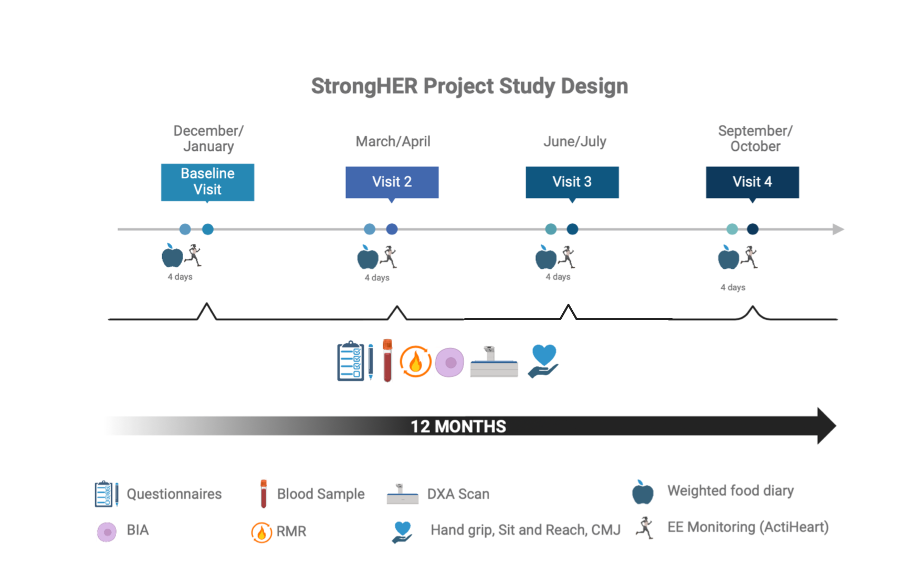
\includegraphics[keepaspectratio]{/Users/Katriona/Documents/Uni/PhD/Thesis/Thesis/studydesign.png}}
\caption{StrongHER Study Design}
\end{figure}

\subsection{Participants}\label{participants}

Participants will be female, aged between \textgreater18 and \textless40 years. Participants will be defined as healthy as determined by a health screening questionnaire. No use of medication that could affect bone metabolism such as glucocorticoids (e.g., prednisone, cortisone). Participants exceeding the weight limit for the DXA scanner will be excluded (\textgreater204kg/450lbs). Further exclusion criteria include any females who are currently pregnant or participants who have breastfed within the last 12 months. Participants' training status will be classified using the criteria outlined by McKay et al. (2021) with supporting classification provided. Participants will be Tier 3 (National level/highly trained) and above. Participants menstrual status will be reported in line with the tiering system proposed by Elliott-Sale et al. (2021). All participants will receive a participant information sheet via email and have a minimum of 24 hours to read through the information sheet. Participants will then be given the opportunity to ask questions prior to providing written informed consent.

\subsection{Ethics}\label{ethics}

Ethical approval was approved by the Energy, Geoscience, Infrastructure and Society Ethics Committee of Heriot Watt University (Dec 2024).

\subsection{Energy Availability \& Energy Expenditure Tracking}\label{energy-availability-energy-expenditure-tracking}

Prior to attending for baseline screening, participants will be asked to visit the lab to have the ActiHeart device correctly fitted. It is vital that the surface of skin is correctly prepared prior to attaching the Actiheart electrodes and before the start of any recording. Manufacturer recommendations will be followed to properly prepare the skin using cardio prep pads. One electrode will be adhered at V1 or V2 (4th intercostals), and the second electrode placed approximately 10cm away on the left side at V4 or V5 although this placement will be adjusted to be comfortable for the subject. Monitors will initially be placed by a research team member and the location of the electrode circled with a permanent marker to ensure accurate replacement of electrodes by participants as needed. The Actiheart software contains an inbuilt signal test function which will be used to check the quality of the R wave signal before commencing recording. Each participant will be provided with their own diet diary via Cronometer and digital food scale. Cronometer will provide a blinded diary, as such it will only allow participants to input data but receive no analysis of foods consumed or feedback of daily targets. Verbal and written instructions detailing how to weigh and record all foods consumed will be given. At this stage, participants will also be asked to complete all initial questionnaires described in section 4.6 and ask any questions they may have.
Short-term EA will be estimated based on dietary and training records following Loucks et al., (2011). The Actiheart monitor is a lightweight and waterproof device that combines both HR measurement and a movement sensor (accelerometery) to provide estimations of daily physical activity levels in a non-invasive manner. Actiheart monitors have shown good levels of agreement with indirect calorimetry during daily living activities in males and females both in laboratory (D. Thompson et al., 2006) and free-living settings (Crouter et al., 2008). Following advice from manufacturers and considering both participant and researcher burden no individual calibration of the devices was completed. The primary outcomes derived from the Actiheart analysis will include both energetic and cardiovascular measures. Specifically, the energetic outcomes will be reported as total energy expenditure, quantified in kilojoules (kJ) and kilocalories (kcal), for each participant. Additionally, the cardiovascular outcomes will be assessed by analysing the time spent in five distinct heart rate zones, defined as percentages of the individuals maximum heart rate. These zones will provide a comprehensive view of them participants physical activity intensity and cardiovascular exertion throughout the monitoring period.
EI will be determined using weighted food diaries over a minimum non-consecutive 4-day period (to include at least one weekend day). Participants will use the mobile application Cronometer (Cronometer, Canada) to input their dietary intake for the research study. Settings will be configured to ensure participants cannot see live intake analysis (e.g.~macronutrient breakdown), rendering their end as a simple data collection form through an app. This aims to reduce underreporting for fear of external judgement and blinds participants to their individualised targets that would typically be provided by similar applications based on personal data. For the remaining visits, participants will be asked to attend the lab at least one week prior to their main visit for device fitting and food diary collection. This will also give the research team an opportunity to ensure recording is as accurate as possible and collect more data if required. Once the appropriate data has been collected participants will be invited to the lab for the next visit to return food scales and have the Actiheart device removed by a member of the research team. Participants will then be asked to complete the full testing protocol outlined above as part of the visit.

\subsection{Baseline Screening}\label{baseline-screening}

Participants will be asked to attend the lab between 0830 and 1000 for a baseline visit. Participants will be asked to attend after a rest day to ensure no residual EEE carries over from the previous day. This involves refraining from intense physical activity in the 12 hours prior to testing (no activity resulting in more than 50\% of maximal HR, American Heart Association). Additionally, participants will be asked to arrive at the lab after \textgreater7 hour fast and having refrained from caffeine and nicotine and other stimulants for \textgreater24 hours prior to assessment (Fullmer et al. 2015). Basic anthropometric measurements including height and body mass will be collected via BIA using the mBCA 555 device (SECA, UK). This device will also be used to measure body composition and phase angle (PhA). Participants will be required to sit in a calm and relaxed manner for \textasciitilde20 minutes prior to RMR testing to allow a steady state to be achieved. COSMED Quark RMR Canopy Hood (Cosmed, Rome, Italy) has been shown to be valid for RMR measurements at rest in both healthy and overweight populations (Blond et al. 2011). The device will be calibrated according to manufacturers' guidelines before each measurement. After calibration, the canopy hood will be placed over the participants head and they will remain in the supine position and instructed to limit talking, movement and avoid sleeping while the test is conducted. If uncomfortable at any point, participants will be encouraged to raise their hand and indicate this to the researchers. Each RMR measurement will be conducted for 25 minutes. The first 5 minutes of data collected will be discarded as participant get used to breathing under the canopy. The Weir equation will be used to determine energy expended (Weir 1949).

\textbf{\(\boldsymbol{\text{RMR(kcal/24hr)} = ((3.94 \times VO_2) + (1.106 \times VCO_2)) \times 1.44}\)}

DXA scans will be completed (See section \ref{physical-testing} for full measurement protocol). Baseline measurements of energy intake and energy expenditure will be collected using weighted food diaries and Actiheart monitoring devices. These will be fully explained and attached to participants following written informed consent during the baseline visit (See section \ref{menstrual-status} for full measurement protocol).

\subsection{Questionnaires}\label{questionnaires}

Participants will receive a Physical Activity Readiness Questionnaire (PAR-Q) (\hyperref[appendix-parq]{See Appendix 1}) for inclusion/exclusion criteria and a screening questionnaire to determine their current health, nutrition and training demands. It will include information on sporting career, when participants started training properly, how long have they been training like this and weekly training load (\hyperref[appendix-training]{See Appendix 2}). Participants will also complete a LEAF-Q. LEAF-Q, Menstrual status and menstrual cycle symptoms will be assessed at each visit.

\subsection{Physical Testing}\label{physical-testing}

\textbf{Muscular strength:} A hand grip dynamometer will be used to measure muscular strength. Model T.K.K.5401 GRIP-D handgrip dynamometer (Takei Scientific Instruments Co., Ltd, Tokyo, Japan) The Takei has been found to be a valid and reliable tool to measure power grip (Teslim and Balogun 1991). Although there is no standard protocol for all dynamometers, there is clear criteria to be followed. Three repetitions per hand, allowing the participant to perform without strict instructions, minimum of 2s hold per repetition and consistent arm position maintained for all repetitions (Gatt et al. 2018). As such, the protocol demonstrated by Amaral et al.(2012) will be used in this study. Instrument specific warm up exercises will be used prior to any maximal contractions. Participants will complete three maximal isometric efforts in the dominant hand with verbal encouragement from the researcher to ensure maximum force. These will be held for 6 seconds with an interval of 2 minutes between them to avoid accumulated muscle fatigue. The participant will be in the standardised American Society of Hand Therapists (ASHT) position (Fess 1992), seated comfortably, shoulder adducted with no rotation, forearm flexed to 90 degrees, wrist position from 0-30 degrees. To standardise grip strength regardless of hand size of participants, the size of the handle will be adjusted to ensure the distal interphalangeal joint of the fifth finger is over the anterior aspect of the handle. All measurements will be completed using the dominant hand for consistency across participants. The mean of the three measurements will be recorded.

\textbf{Flexibility:} Classic Sit and reach test (CSR) will be used to measure flexibility in the hamstrings. A valid and reliable tool that is easy to administer and low-cost (Mayorga-Vega, Merino-Marban, and Viciana 2014). The SR requires participants to place the soles of their feet at the base of the SR box, straighten their legs and sit as upright as possible. The participant will be asked to place one hand on top of the other and slowly touch a point as far in front of them as possible. Movement will be repeated three times and the highest value of the three tests will be recorded (French et al. 2016).

\textbf{CMJ:} Counter-movement jumps (CMJ) without arm-swing will be performed. To standardise jump tests, participants will be instructed to perform all attempts in accordance with the protocol outlined in Wilson-Barnes et al.(2021). Movement specific warm-ups will be completed with participants completing two jumps at 50\% and 80\% effort prior to starting to ensure correct technique. For the test, three attempts will be performed with hands on hips, and the best result will be recorded in centimetres (cm) for further analysis. A recovery interval of 1-min between jumps will be provided. The Optojump (Microgate., NY) will be used which has been previously validated (Glatthorn et al. 2011; Rago et al. 2018).

\subsection{DXA Scans}\label{dxa-scans}

DXA scans will be performed by trained technicians using Hologic Horizon DXA System (Hologic BVBA., Zaventem, Belgium). DXA scans will provide anthropometric data including:

\begin{itemize}
\tightlist
\item
  \textbf{Fat mass (FM)}
\item
  \textbf{Lean mass (LM)}
\item
  \textbf{Fat mass index (FMI) - Fat mass divided by height\textsubscript{2}}
\item
  \textbf{Lean Mass Index (LMI) - Lean mass divided by height\textsubscript{2}}
\item
  \textbf{Bone mineral content (BMC)}
\item
  \textbf{Bone mineral density (BMD)}
\item
  \textbf{Android/Gynoid ratio}
\item
  \textbf{Fat mass ratio (FMR) - upper body vs legs}
\item
  \textbf{Trunk vs Limb fat mass ratio (TFMR) - upper body vs legs \& arms combined}
\end{itemize}

BMD Z-scores will be used as a comparison of sex and age matched controls (recommended by ISCD) at the lumbar spine and hip. The hip is the most reliable measure for predicting hip fracture risk; the spine for monitoring changes in bone density (Blake and Fogelman 2007). The DEXA will also provide data to check the homogeneity of the group and associations between adiposity and bone health.

\subsection{Bioelectrical Impedance Analysis (BIA)}\label{bioelectrical-impedance-analysis-bia}

Participants will also be asked to empty their bladder 30 minutes before the test. Any metallic accessories or jewellery will be removed to avoid interference with the measurement. Participants will be asked to stand barefoot on the BIA device platform and instructed to hold the handrails with fixed handle positions, ensuring proper contact with the electrodes embedded in the handrails. The mBCA 555 (SECA, UK) device will pass a low, safe electrical current through the body. The device measures the resistance (R) and reactance (Xc) of body tissues to the current.
These measurements are then used to calculate the phase angle using the formula below:

\(\mathbf{Arctangent} \left( \frac{\mathbf{Xc}}{\mathbf{R}} \right) \times \frac{180}{\pi}\)

Each measurement will be recorded in duplicate to ensure reliability, with a brief interval between measurements. A third measurement will be completed if variances are seen outside of accepted ranges. The average of the measurements will be used for analysis.

\subsection{Venous Blood Samples}\label{venous-blood-samples}

Venous blood samples will be collected by a trained phlebotomist. All blood samples will be collected via venepuncture from an antecubital vein with the participant seated on a laboratory bed. For plasma, whole blood will be centrifuged at 1500 rpm for 15 min at 4°C within 30 min of collection. For serum, whole blood will be incubated at room temperature for 30 min prior to centrifugation at 1000 x g for 10 min at 4°C. The resulting plasma and serum will be aliquoted into 1.5 ml vials and stored at minus 80°C for subsequent analysis.

\subsection{Blood Sample Analysis}\label{blood-sample-analysis}

Samples will be collected for total serum 25(OH)D3, calcium, and Free 25(OH)D. Free 25(OH)D will be calculated using the equation below (Bikle et al. 1986), where free 25(OH)D = concentration of free 25(OH) vitamin D in mol/L, K\textsubscript{alb} = affinity constant (K\textsubscript{alb} = 6 × 105 M\textsuperscript{−1}) between 25(OH) vitamin D and albumin in mol\textsuperscript{−1}, K\textsubscript{DBP} = affinity constant (K\textsubscript{DBP} = 7 × 108 M\textsuperscript{−1}) between 25(OH) vitamin D and DBP in mol−1, albumin = concentration of total serum albumin in mol/L, DBP = concentration of total vitamin D-binding protein in mol/L and total 25(OH) vitamin D = concentration of total 25(OH)D in mol/L.

\textbf{Free 25(OH)D = total 25(OH)D/1+ (K\textsubscript{alb} x albumin) + (K\textsubscript{DBP} x DBP)}

We will also calculate the `bioavailable portion' using the following equation:

\textbf{Bioavailable 25(OH)D = (K\textsubscript{alb} × albumin)+1) × Free 25(OH)D}

Parathyroid hormone (PTH) will also be measured. To assess MC phase, serum estrogen and progesterone will be measured. To assess LEA and the impact on the female athlete this study will measure Triiodothyronine (T3), leptin, grehlin (acylated and desacylated) and insulin. Specific bone turnover markers will also be included with one marker of both formation and resorption. These markers will include P1NP and C terminal telopeptide of type 1 collagen (CTX) as these are some of the most sensitive markers and are often used to monitor anti-resorptive therapies in people with low bone mass.

\subsection{Menstrual Status}\label{menstrual-status}

Menstrual status (MS) will be assessed via questionnaire (\hyperref[appendix-menstrualq]{See Appendix 3}). Menstrual cycle (MC) phase will be assessed using calendar-based counting and venous blood samples to determine both estrogen and progesterone concentrations. To be classified as naturally menstruating participants will (1) have MC lengths ≥ 21 days and ≤ 35 days resulting in nine or more consecutive periods per year; (2) have not used any type of hormonal contraceptive for a minimum of 3 months, but ideally 6 months, before enrolment. MC phase tracking will be achieved by denoting the first and last day of menstruation for each cycle and informing the primary researcher by email.

\subsection{Menstrual Cycle Symptoms Tracking}\label{menstrual-cycle-symptoms-tracking}

Menstrual cycle symptom assessment will be completed on each visit to the laboratory. Participants will be asked to complete a questionnaire to recall their symptoms from their most recent cycle (Appendix 3). This will include information on the presence/absence of a MC, frequency, severity of symptoms and impact on training. The questionnaire is adapted from Oslo Sports Trauma Research Centre (OSTRC) Overuse Injury Questionnaire (Clarsen, Myklebust, and Bahr 2013).

\section{Statistical Analysis}\label{statistical-analysis}

\subsection{Descriptive}\label{descriptive}

\begin{enumerate}
\def\labelenumi{\arabic{enumi}.}
\item
  Descriptive statistics (mean, standard deviation, median, and range) for variables such as anthropometric measurements (height, body mass), serum vitamin D levels, calcium levels, bioavailable vitamin D levels, and DEXA scan results (fat mass, lean mass, z-scores).
\item
  Calculate frequency distributions for categorical variables including menstrual function categories, participant training status, and EA categories.
\end{enumerate}

\subsection{Statistical}\label{statistical}

Independent Samples t-tests:
1. Compare mean differences in bone health markers between different categories of participant, such as athletes with vitamin D deficiency versus those with sufficient levels.

Analysis of Variance (ANOVA \& ANCOVA)
2. Assess variations in bone turnover markers and EA across different sports.

\subsection{Linear Regression}\label{linear-regression}

\begin{enumerate}
\def\labelenumi{\arabic{enumi}.}
\tightlist
\item
  Investigate the relationship between EA and bone turnover markers
\end{enumerate}

\subsection{Correlations}\label{correlations}

Pearson Correlation Coefficients:
1. Examine the correlations between continuous variables, such as the relationship between serum vitamin D levels and bone turnover markers.

Repeated Measures Analysis of Variance (ANOVA):
1. Explore changes in EA, bone turnover markers, micronutrient status over the repeated measures across the 12-month period.

Multivariate Analysis of Variance (MANOVA):
2. Analyse the combined effect of training status, vitamin D levels on bone turnover markers.

\section{Expected Outcomes}\label{expected-outcomes-1}

In conclusion, the proposed longitudinal observational study exploring female athlete bone health, EA, and micronutrient intakes holds substantial implications for advancing our understanding of the intricate relationship between EA, micronutrient status, and bone health in female athletes. By addressing critical gaps in existing knowledge, the research aims to inform evidence-based guidelines, tailor interventions to the unique needs of female athletes, and optimise both their health and performance outcomes. The study's potential impact extends beyond academia, providing practical insights for coaches, sports nutritionists, and healthcare professionals involved in the care of female athletes living in Scotland. The dissemination strategy includes publishing findings in peer-reviewed journals such as British Journal of Sports Medicine, International Journal of Sports Nutrition and Exercise Metabolism and Journal of the International Society of Sports Nutrition. Findings will also be presented at academic and professional conferences, conducting workshops with relevant stakeholders where possible. Additionally, once complete participants will be able to receive feedback on their own data ensuring they are informed of any relevant findings that may impact their training, nutrition or long term-health. This research aims to enhance the quality of female-specific data, contributing to a more nuanced understanding of the unique physiological considerations affecting female athlete health and performance.

\section{References}\label{references}

\appendix


\subsection{Appendix 1: PAR-Q Questionnaire}\label{appendix-parq}

\subsection{Appendix 2: Training and Nutrition Questionnaire}\label{appendix-training}

\subsection{Appendix 3: Menstrual Status \& Symptoms Questionnaire}\label{appendix-menstrualq}

\textbf{\underline{Menstrual status and menstrual cycle related symptoms}}

This questionnaire is going to ask you about your menstrual status,
your experience of menstrual cycle related symptoms and how you
feel that these symptoms impact your training and competition. 

If you do not feel comfortable answering any of the questions you can
leave them blank.

\textbf{\underline{Menstrual status}}

\begin{enumerate}
\def\labelenumi{\arabic{enumi})}
\item
  Have you had your first period?
\end{enumerate}

Yes No (\textbf{skip to Q9}) Prefer not to say

\begin{enumerate}
\def\labelenumi{\alph{enumi}.}
\item
  At what age did you have your first period (years)?
\end{enumerate}

\begin{quote}
years old Prefer not to say
\end{quote}

\begin{enumerate}
\def\labelenumi{\arabic{enumi})}
\setcounter{enumi}{1}
\item
  On average, would you consider yourself to have a regular menstrual
  cycle length (days between a period)? \emph{In the UK the average
  length of a cycle is between 21-35 days.}
\end{enumerate}

\begin{quote}
Yes No Don't know Prefer not to say
\end{quote}

\begin{enumerate}
\def\labelenumi{\arabic{enumi})}
\setcounter{enumi}{2}
\item
  Have you had a period within the last 3 months?
\end{enumerate}

\begin{quote}
Yes No Prefer not to say
\end{quote}

\begin{enumerate}
\def\labelenumi{\alph{enumi}.}
\item
  If no to Q3, do you know of any reason why you have not had a period
  in the last 3 months? (e.g. pregnancy, surgery or other)
\end{enumerate}

Yes No Prefer not to say

\begin{enumerate}
\def\labelenumi{\alph{enumi}.}
\setcounter{enumi}{1}
\item
  If yes to Q3a, please provide details if you feel comfortable to:
\end{enumerate}

\begin{longtable}[]{@{}
  >{\raggedright\arraybackslash}p{(\linewidth - 0\tabcolsep) * \real{1.0000}}@{}}
\toprule\noalign{}
\begin{minipage}[b]{\linewidth}\raggedright
\end{minipage} \\
\midrule\noalign{}
\endhead
\bottomrule\noalign{}
\endlastfoot
\end{longtable}

\begin{enumerate}
\def\labelenumi{\arabic{enumi})}
\setcounter{enumi}{3}
\item
  Over the last 3 months, would you consider yourself to have a regular
  menstrual cycle length (days between a period)? In the UK average
  length of a cycle is between 21-35 days.
\end{enumerate}

Yes No Don't know Prefer not to say

\begin{enumerate}
\def\labelenumi{\arabic{enumi})}
\setcounter{enumi}{4}
\item
  On average how long does your period (days bleeding) last?
\end{enumerate}

0-2 days 3-4 days 5-7 days 7+ days Not applicable

\begin{enumerate}
\def\labelenumi{\arabic{enumi})}
\setcounter{enumi}{5}
\item
  Do you currently use any form of hormonal (e.g., contraceptive pill,
  injection, implant, vaginal ring, hormonal intrauterine system) or
  non-hormonal contraceptive (e.g., copper coil)?
\end{enumerate}

Yes No Prefer not to say

\begin{enumerate}
\def\labelenumi{\arabic{enumi})}
\setcounter{enumi}{6}
\item
  If yes, what type of contraceptive do you use? Where possible please
  give type, brand and how you take this e.g., I take a placebo pill, I
  take active pills back-to-back. If you are unsure how to answer this
  or need any guidance please ask a researcher.
\end{enumerate}

\begin{longtable}[]{@{}
  >{\raggedright\arraybackslash}p{(\linewidth - 0\tabcolsep) * \real{1.0000}}@{}}
\toprule\noalign{}
\begin{minipage}[b]{\linewidth}\raggedright
\end{minipage} \\
\midrule\noalign{}
\endhead
\bottomrule\noalign{}
\endlastfoot
\end{longtable}

\begin{enumerate}
\def\labelenumi{\arabic{enumi})}
\setcounter{enumi}{7}
\item
  Do you use a non-hormonal copper intrauterine system?
\end{enumerate}

Yes No Prefer not to say

\begin{enumerate}
\def\labelenumi{\arabic{enumi})}
\setcounter{enumi}{8}
\item
  Is there anything that we have not asked that you think we should know
  or anything you would like to clarify (optional answer box)?
\end{enumerate}

(e.g., I have gone from not using a contraceptive to taking a progestin
only contraceptive 2 weeks ago, I have stopped using my combined pill 2
months ago, I have been told I have polycystic ovary syndrome (PCOS), I
have been told I have endometriosis, etc.)

\_\_\_\_\_\_\_\_\_\_\_\_\_\_\_\_\_\_\_\_\_\_\_\_\_\_\_\_\_\_\_\_\_\_\_\_\_\_\_\_\_\_\_

\textbf{\underline{Menstrual cycle related symptoms}}

\begin{enumerate}
\def\labelenumi{\arabic{enumi})}
\setcounter{enumi}{9}
\item
  In the last 3 months, have you experienced any of the following
  symptoms throughout your menstrual cycle? For each symptom, please
  rate the frequency and severity of symptoms and indicate how much you
  feel that they impact you in training or competition.
\end{enumerate}

\begin{quote}
If you answer ``Never'' for frequency you do not need to fill in the
columns for severity, impact on training or impact on competition for
this symptom.
\end{quote}

\begin{longtable}[]{@{}
  >{\raggedright\arraybackslash}p{(\linewidth - 36\tabcolsep) * \real{0.1723}}
  >{\raggedright\arraybackslash}p{(\linewidth - 36\tabcolsep) * \real{0.0456}}
  >{\raggedright\arraybackslash}p{(\linewidth - 36\tabcolsep) * \real{0.0456}}
  >{\raggedright\arraybackslash}p{(\linewidth - 36\tabcolsep) * \real{0.0458}}
  >{\raggedright\arraybackslash}p{(\linewidth - 36\tabcolsep) * \real{0.0464}}
  >{\raggedright\arraybackslash}p{(\linewidth - 36\tabcolsep) * \real{0.0460}}
  >{\raggedright\arraybackslash}p{(\linewidth - 36\tabcolsep) * \real{0.0458}}
  >{\raggedright\arraybackslash}p{(\linewidth - 36\tabcolsep) * \real{0.0460}}
  >{\raggedright\arraybackslash}p{(\linewidth - 36\tabcolsep) * \real{0.0458}}
  >{\raggedright\arraybackslash}p{(\linewidth - 36\tabcolsep) * \real{0.0458}}
  >{\raggedright\arraybackslash}p{(\linewidth - 36\tabcolsep) * \real{0.0460}}
  >{\raggedright\arraybackslash}p{(\linewidth - 36\tabcolsep) * \real{0.0458}}
  >{\raggedright\arraybackslash}p{(\linewidth - 36\tabcolsep) * \real{0.0460}}
  >{\raggedright\arraybackslash}p{(\linewidth - 36\tabcolsep) * \real{0.0462}}
  >{\raggedright\arraybackslash}p{(\linewidth - 36\tabcolsep) * \real{0.0458}}
  >{\raggedright\arraybackslash}p{(\linewidth - 36\tabcolsep) * \real{0.0460}}
  >{\raggedright\arraybackslash}p{(\linewidth - 36\tabcolsep) * \real{0.0458}}
  >{\raggedright\arraybackslash}p{(\linewidth - 36\tabcolsep) * \real{0.0472}}
  >{\raggedright\arraybackslash}p{(\linewidth - 36\tabcolsep) * \real{0.0460}}@{}}
\toprule\noalign{}
\multirow{2}{*}{\begin{minipage}[b]{\linewidth}\centering Content\end{minipage}} & 
\textbf{Symptom} &
\multicolumn{4}{>{\raggedright\arraybackslash}p{(\linewidth - 36\tabcolsep) * \real{0.1835} + 6\tabcolsep}}{%
\begin{minipage}[b]{\linewidth}\raggedright \textbf{Frequency} \end{minipage}} &
\multicolumn{4}{>{\raggedright\arraybackslash}p{(\linewidth - 36\tabcolsep) * \real{0.1835} + 6\tabcolsep}}{%
\begin{minipage}[b]{\linewidth}\raggedright
\textbf{Frequency}
\end{minipage}} &
\multicolumn{4}{>{\raggedright\arraybackslash}p{(\linewidth - 36\tabcolsep) * \real{0.1836} + 6\tabcolsep}}{%
\begin{minipage}[b]{\linewidth}\raggedright
\textbf{Severity}
\end{minipage}} &
\multicolumn{5}{>{\raggedright\arraybackslash}p{(\linewidth - 36\tabcolsep) * \real{0.2298} + 8\tabcolsep}}{%
\begin{minipage}[b]{\linewidth}\raggedright
\textbf{Impact on training}
\end{minipage}} &
\multicolumn{5}{>{\raggedright\arraybackslash}p{(\linewidth - 36\tabcolsep) * \real{0.2308} + 8\tabcolsep}@{}}{%
\begin{minipage}[b]{\linewidth}\raggedright
\textbf{Impact on competition}
\end{minipage}} \\
& \begin{minipage}[b]{\linewidth}\centering
\begin{quote}
\textbf{Never}
\end{quote}
\end{minipage} & \begin{minipage}[b]{\linewidth}\centering
\begin{quote}
\textbf{Rarely}
\end{quote}
\end{minipage} & \begin{minipage}[b]{\linewidth}\centering
\begin{quote}
\textbf{Sometimes}
\end{quote}
\end{minipage} & \begin{minipage}[b]{\linewidth}\centering
\begin{quote}
\textbf{Often}
\end{quote}
\end{minipage} & \begin{minipage}[b]{\linewidth}\centering
\begin{quote}
\textbf{Absent}
\end{quote}
\end{minipage} & \begin{minipage}[b]{\linewidth}\centering
\begin{quote}
\textbf{Mild}
\end{quote}
\end{minipage} & \begin{minipage}[b]{\linewidth}\centering
\begin{quote}
\textbf{Moderate}
\end{quote}
\end{minipage} & \begin{minipage}[b]{\linewidth}\centering
\begin{quote}
\textbf{Severe}
\end{quote}
\end{minipage} & \begin{minipage}[b]{\linewidth}\centering
\begin{quote}
\textbf{No impact}
\end{quote}
\end{minipage} & \begin{minipage}[b]{\linewidth}\centering
\begin{quote}
\textbf{To a minor extent}
\end{quote}
\end{minipage} & \begin{minipage}[b]{\linewidth}\centering
\begin{quote}
\textbf{To a moderate extent}
\end{quote}
\end{minipage} & \begin{minipage}[b]{\linewidth}\centering
\begin{quote}
\textbf{To a major extent}
\end{quote}
\end{minipage} & \begin{minipage}[b]{\linewidth}\centering
\begin{quote}
\textbf{Cannot participate at all}
\end{quote}
\end{minipage} & \begin{minipage}[b]{\linewidth}\centering
\begin{quote}
\textbf{No impact}
\end{quote}
\end{minipage} & \begin{minipage}[b]{\linewidth}\centering
\begin{quote}
\textbf{To a minor extent}
\end{quote}
\end{minipage} & \begin{minipage}[b]{\linewidth}\centering
\begin{quote}
\textbf{To a moderate extent}
\end{quote}
\end{minipage} & \begin{minipage}[b]{\linewidth}\centering
\begin{quote}
\textbf{To a major extent}
\end{quote}
\end{minipage} & \begin{minipage}[b]{\linewidth}\centering
\begin{quote}
\textbf{Cannot participate at all}
\end{quote}
\end{minipage} \\
\midrule\noalign{}
\endhead
\bottomrule\noalign{}
\endlastfoot
\multicolumn{19}{@{}>{\raggedright\arraybackslash}p{(\linewidth - 36\tabcolsep) * \real{1.0000} + 36\tabcolsep}@{}}{%
Physical symptoms} \\
Changes to breathing & & & & & & & & & & & & & & & & & & \\
Difficulties in breathing & & & & & & & & & & & & & & & & & & \\
Nausea & & & & & & & & & & & & & & & & & & \\
Sickness or vomiting & & & & & & & & & & & & & & & & & & \\
Constipation & & & & & & & & & & & & & & & & & & \\
Dizziness & & & & & & & & & & & & & & & & & & \\
Light headedness & & & & & & & & & & & & & & & & & & \\
Reduced coordination & & & & & & & & & & & & & & & & & & \\
Joint pain & & & & & & & & & & & & & & & & & & \\
Muscle aches & & & & & & & & & & & & & & & & & & \\
Muscle cramps & & & & & & & & & & & & & & & & & & \\
Temperature fluctuations & & & & & & & & & & & & & & & & & & \\
Night sweats & & & & & & & & & & & & & & & & & & \\
Disturbed sleep & & & & & & & & & & & & & & & & & & \\
Increased sleep duration & & & & & & & & & & & & & & & & & & \\
Diarrhoea & & & & & & & & & & & & & & & & & & \\
Headaches & & & & & & & & & & & & & & & & & & \\
Migraines & & & & & & & & & & & & & & & & & & \\
Lower back pain & & & & & & & & & & & & & & & & & & \\
Water retention & & & & & & & & & & & & & & & & & & \\
Bloating & & & & & & & & & & & & & & & & & & \\
Increased gas & & & & & & & & & & & & & & & & & & \\
Stomach pain (sometimes called cramps) & & & & & & & & & & & & & & & & &
& \\
Tiredness & & & & & & & & & & & & & & & & & & \\
Fatigue & & & & & & & & & & & & & & & & & & \\
Breast pain & & & & & & & & & & & & & & & & & & \\
Breast tenderness & & & & & & & & & & & & & & & & & & \\
Food cravings & & & & & & & & & & & & & & & & & & \\
Changes in appetite & & & & & & & & & & & & & & & & & & \\
Heavy bleeding & & & & & & & & & & & & & & & & & & \\
Flooding from period & & & & & & & & & & & & & & & & & & \\
Cold symptoms (e.g., sneezing, sore throat, etc.) & & & & & & & & & & &
& & & & & & & \\
Feeling weak & & & & & & & & & & & & & & & & & & \\
Feeling slow & & & & & & & & & & & & & & & & & & \\
\multicolumn{18}{@{}>{\raggedright\arraybackslash}p{(\linewidth - 36\tabcolsep) * \real{0.9540} + 34\tabcolsep}}{%
Psychological symptoms} & \\
Mood changes & & & & & & & & & & & & & & & & & & \\
Irritability & & & & & & & & & & & & & & & & & & \\
Anxiety & & & & & & & & & & & & & & & & & & \\
Low motivation & & & & & & & & & & & & & & & & & & \\
Reduced concentration & & & & & & & & & & & & & & & & & & \\
Reduced focus & & & & & & & & & & & & & & & & & & \\
Feeling sad or depressed & & & & & & & & & & & & & & & & & & \\
\multicolumn{19}{@{}>{\raggedright\arraybackslash}p{(\linewidth - 36\tabcolsep) * \real{1.0000} + 36\tabcolsep}@{}}{%
Other symptoms (if there are any symptoms we have not listed here that
you would like to tell us about please list them below):} \\
& & & & & & & & & & & & & & & & & & \\
& & & & & & & & & & & & & & & & & & \\
& & & & & & & & & & & & & & & & & & \\
& & & & & & & & & & & & & & & & & & \\
& & & & & & & & & & & & & & & & & & \\
\end{longtable}

\begin{enumerate}
\def\labelenumi{\arabic{enumi})}
\setcounter{enumi}{10}
\item
  Over the last 3 months, to what extent have you reduced your training
  volume due to any menstrual cycle related symptoms?
\end{enumerate}

No reduction

To a minor extent

To a moderate extent

To a major extent

Could not participate at all

\begin{enumerate}
\def\labelenumi{\arabic{enumi})}
\setcounter{enumi}{11}
\item
  Over the last 3 months, to what extent have any menstrual cycle
  related symptoms affected your performance?
\end{enumerate}

\begin{quote}
No effect

To a minor extent

To a moderate extent

To a major extent

Could not participate at all
\end{quote}

\begin{enumerate}
\def\labelenumi{\arabic{enumi})}
\setcounter{enumi}{12}
\item
  Throughout your menstrual cycle or while taking your contraceptive, do
  you notice any positive symptoms (e.g., improved mood at certain
  phases, increased flexibility, better focus)?
\end{enumerate}

\begin{quote}
Yes No Prefer not to say
\end{quote}

\begin{enumerate}
\def\labelenumi{\alph{enumi}.}
\item
  If yes, what positive symptoms do you experience? Provide as much
  details as you feel comfortable to.
\end{enumerate}

\begin{longtable}[]{@{}
  >{\raggedright\arraybackslash}p{(\linewidth - 0\tabcolsep) * \real{1.0000}}@{}}
\toprule\noalign{}
\begin{minipage}[b]{\linewidth}\raggedright
\end{minipage} \\
\midrule\noalign{}
\endhead
\bottomrule\noalign{}
\endlastfoot
\end{longtable}

\begin{enumerate}
\def\labelenumi{\arabic{enumi})}
\setcounter{enumi}{13}
\item
  Do you take any medication to manage your menstrual cycle related
  symptoms (e.g., ibuprofen, paracetamol)?
\end{enumerate}

\begin{quote}
Yes No Prefer not to say
\end{quote}

\begin{enumerate}
\def\labelenumi{\alph{enumi}.}
\item
  If yes to Q13, please provide details if you feel comfortable to:
\end{enumerate}

\begin{longtable}[]{@{}
  >{\raggedright\arraybackslash}p{(\linewidth - 0\tabcolsep) * \real{1.0000}}@{}}
\toprule\noalign{}
\begin{minipage}[b]{\linewidth}\raggedright
\end{minipage} \\
\midrule\noalign{}
\endhead
\bottomrule\noalign{}
\endlastfoot
\end{longtable}

\begin{enumerate}
\def\labelenumi{\arabic{enumi})}
\setcounter{enumi}{14}
\item
  Do you take any nutritional supplements to manage your menstrual cycle
  related symptoms (e.g., vitamin D, omega-3, etc.)?
\end{enumerate}

\begin{quote}
Yes No Prefer not to say
\end{quote}

\begin{enumerate}
\def\labelenumi{\alph{enumi}.}
\item
  If yes to Q14, please provide details if you feel comfortable to:
\end{enumerate}

\begin{longtable}[]{@{}
  >{\raggedright\arraybackslash}p{(\linewidth - 0\tabcolsep) * \real{1.0000}}@{}}
\toprule\noalign{}
\begin{minipage}[b]{\linewidth}\raggedright
\end{minipage} \\
\midrule\noalign{}
\endhead
\bottomrule\noalign{}
\endlastfoot
\end{longtable}

\begin{enumerate}
\def\labelenumi{\arabic{enumi})}
\setcounter{enumi}{15}
\item
  Do you do anything else to manage your menstrual cycle related
  symptoms (e.g., tens machine, hot water bottle)?
\end{enumerate}

\begin{quote}
Yes No Prefer not to say
\end{quote}

\begin{enumerate}
\def\labelenumi{\alph{enumi}.}
\item
  If yes to Q15, please provide details if you feel comfortable to:
\end{enumerate}

\begin{longtable}[]{@{}
  >{\raggedright\arraybackslash}p{(\linewidth - 0\tabcolsep) * \real{1.0000}}@{}}
\toprule\noalign{}
\begin{minipage}[b]{\linewidth}\raggedright
\end{minipage} \\
\midrule\noalign{}
\endhead
\bottomrule\noalign{}
\endlastfoot
\end{longtable}

\begin{enumerate}
\def\labelenumi{\arabic{enumi})}
\setcounter{enumi}{16}
\item
  Have you had any previous education about your menstrual cycle or
  contraceptive use sports performance?
\end{enumerate}

\begin{quote}
Yes No Prefer not to say
\end{quote}

\begin{enumerate}
\def\labelenumi{\arabic{enumi})}
\setcounter{enumi}{17}
\item
  Do you talk to you currently talk with your coach or any support staff
  about your menstrual cycle or contraceptive use?
\end{enumerate}

Yes No Prefer not to say

\begin{enumerate}
\def\labelenumi{\alph{enumi}.}
\item
  If no, would you feel comfortable talking to your coach or any support
  staff about your menstrual cycle or contraceptive use?
\end{enumerate}

\begin{quote}
Yes No Prefer not to say
\end{quote}


bookdown::render\_book(``Thesis.Rmd'', ``bookdown::gitbook'')

\phantomsection\label{refs}
\begin{CSLReferences}{1}{0}
\bibitem[\citeproctext]{ref-alimoradi_efficacy_2019}
Alimoradi, Karamollah, Bahareh Nikooyeh, Ali Asghar Ravasi, Maliheh Zahedirad, Nastaran Shariatzadeh, Ali Kalayi, and Tirang Reza Neyestani. 2019. {``Efficacy of {Vitamin} {D} {Supplementation} in {Physical} {Performance} of {Iranian} {Elite} {Athletes}.''} \emph{International Journal of Preventive Medicine} 10 (June): 100. \url{https://doi.org/10.4103/ijpvm.IJPVM_227_18}.

\bibitem[\citeproctext]{ref-amaral_comparison_2012}
Amaral, Josária F., Marcelly Mancini, and José M. Novo Júnior. 2012. {``Comparison of Three Hand Dynamometers in Relation to the Accuracy and Precision of the Measurements.''} \emph{Revista Brasileira De Fisioterapia (Sao Carlos (Sao Paulo, Brazil))} 16 (3): 216--24. \url{https://doi.org/10.1590/s1413-35552012000300007}.

\bibitem[\citeproctext]{ref-arciero_resting_1993}
Arciero, P. J., M. I. Goran, and E. T. Poehlman. 1993. {``Resting Metabolic Rate Is Lower in Women Than in Men.''} \emph{Journal of Applied Physiology (Bethesda, Md.: 1985)} 75 (6): 2514--20. \url{https://doi.org/10.1152/jappl.1993.75.6.2514}.

\bibitem[\citeproctext]{ref-areta_low_2021}
Areta, José L., Harry L. Taylor, and Karsten Koehler. 2021. {``Low Energy Availability: History, Definition and Evidence of Its Endocrine, Metabolic and Physiological Effects in Prospective Studies in Females and Males.''} \emph{European Journal of Applied Physiology} 121 (1): 1--21. \url{https://doi.org/10.1007/s00421-020-04516-0}.

\bibitem[\citeproctext]{ref-bailey_exercise_2008}
Bailey, C. A., and K. Brooke-Wavell. 2008. {``Exercise for Optimising Peak Bone Mass in Women: {Postgraduate} {Symposium}.''} \emph{Proceedings of the Nutrition Society} 67 (1): 9--18. \url{https://doi.org/10.1017/S0029665108005971}.

\bibitem[\citeproctext]{ref-barrack_higher_2014}
Barrack, Michelle T., Jenna C. Gibbs, Mary Jane De Souza, Nancy I. Williams, Jeanne F. Nichols, Mitchell J. Rauh, and Aurelia Nattiv. 2014. {``Higher {Incidence} of {Bone} {Stress} {Injuries} {With} {Increasing} {Female} {Athlete} {Triad}--{Related} {Risk} {Factors}: {A} {Prospective} {Multisite} {Study} of {Exercising} {Girls} and {Women}.''} \emph{The American Journal of Sports Medicine} 42 (4): 949--58. \url{https://doi.org/10.1177/0363546513520295}.

\bibitem[\citeproctext]{ref-bass_exercise_1998}
Bass, S., G. Pearce, M. Bradney, E. Hendrich, P. D. Delmas, A. Harding, and E. Seeman. 1998. {``Exercise Before Puberty May Confer Residual Benefits in Bone Density in Adulthood: Studies in Active Prepubertal and Retired Female Gymnasts.''} \emph{Journal of Bone and Mineral Research: The Official Journal of the American Society for Bone and Mineral Research} 13 (3): 500--507. \url{https://doi.org/10.1359/jbmr.1998.13.3.500}.

\bibitem[\citeproctext]{ref-berry_vitamin_2011}
Berry, Diane J., Kathryn Hesketh, Chris Power, and Elina Hyppönen. 2011. {``Vitamin {D} Status Has a Linear Association with Seasonal Infections and Lung Function in {British} Adults.''} \emph{British Journal of Nutrition} 106 (9): 1433--40. \url{https://doi.org/10.1017/S0007114511001991}.

\bibitem[\citeproctext]{ref-bezuglov_does_2023}
Bezuglov, Eduard, Maria Shoshorina, Artemii Lazarev, Anton Emanov, Egana Koroleva, Ilsyuyar Anishchenko, Zbigniew Waśkiewicz, Mikhail Butovskiy, and Ryland Morgans. 2023. {``Does Vitamin {D} Affect Strength and Speed Characteristics and Testosterone Concentration in Elite Young Track and Field Athletes in the {North} {European} Summer?''} \emph{Nutrition Journal} 22 (March): 16. \url{https://doi.org/10.1186/s12937-023-00848-7}.

\bibitem[\citeproctext]{ref-bikle_assessment_1986}
Bikle, D. D., E. Gee, B. Halloran, M. A. Kowalski, E. Ryzen, and J. G. Haddad. 1986. {``Assessment of the Free Fraction of 25-Hydroxyvitamin {D} in Serum and Its Regulation by Albumin and the Vitamin {D}-Binding Protein.''} \emph{The Journal of Clinical Endocrinology and Metabolism} 63 (4): 954--59. \url{https://doi.org/10.1210/jcem-63-4-954}.

\bibitem[\citeproctext]{ref-bishop_bone_2021}
Bishop, Meghan E., Alessandra Ahlmen, Jessica Rosendorf, Brandon J. Erickson, and Steven Cohen. 2021. {``Bone Stress Injuries in Female Athletes.''} \emph{Annals of Joint} 6 (0). \url{https://doi.org/10.21037/aoj.2020.04.04}.

\bibitem[\citeproctext]{ref-blake_role_2007}
Blake, Glen M., and Ignac Fogelman. 2007. {``The Role of {DXA} Bone Density Scans in the Diagnosis and Treatment of Osteoporosis.''} \emph{Postgraduate Medical Journal} 83 (982): 509--17. \url{https://doi.org/10.1136/pgmj.2007.057505}.

\bibitem[\citeproctext]{ref-blond_new_2011}
Blond, Emilie, Christine Maitrepierre, Sylvie Normand, Monique Sothier, Hubert Roth, Joelle Goudable, and Martine Laville. 2011. {``A New Indirect Calorimeter Is Accurate and Reliable for Measuring Basal Energy Expenditure, Thermic Effect of Food and Substrate Oxidation in Obese and Healthy Subjects.''} \emph{European e-Journal of Clinical Nutrition and Metabolism} 6 (1): e7--15. \url{https://doi.org/10.1016/j.eclnm.2010.12.001}.

\bibitem[\citeproctext]{ref-brannstrom_vitamin_2016}
Brännström, André, Ji-Guo Yu, Per Jonsson, Torbjörn Akerfeldt, Mats Stridsberg, and Michael Svensson. 2016. {``Vitamin {D} in Relation to Bone Health and Muscle Function in Young Female Soccer Players.''} \emph{European Journal of Sport Science} 17 (September): 1--8. \url{https://doi.org/10.1080/17461391.2016.1225823}.

\bibitem[\citeproctext]{ref-chen_sex_2022}
Chen, Yilin, Minhoo Kim, Sanjana Paye, and Bérénice A. Benayoun. 2022. {``Sex as a {Biological} {Variable} in {Nutrition} {Research}: {From} {Human} {Studies} to {Animal} {Models}.''} \emph{Annual Review of Nutrition} 42 (Volume 42, 2022): 227--50. \url{https://doi.org/10.1146/annurev-nutr-062220-105852}.

\bibitem[\citeproctext]{ref-chu_relationship_2021}
Chu, Chang, Oleg Tsuprykov, Xin Chen, Saban Elitok, Bernhard K. Krämer, and Berthold Hocher. 2021. {``Relationship {Between} {Vitamin} {D} and {Hormones} {Important} for {Human} {Fertility} in {Reproductive}-{Aged} {Women}.''} \emph{Frontiers in Endocrinology} 12 (April). \url{https://doi.org/10.3389/fendo.2021.666687}.

\bibitem[\citeproctext]{ref-clarsen_development_2013}
Clarsen, Benjamin, Grethe Myklebust, and Roald Bahr. 2013. {``Development and Validation of a New Method for the Registration of Overuse Injuries in Sports Injury Epidemiology: The {Oslo} {Sports} {Trauma} {Research} {Centre} ({OSTRC}) {Overuse} {Injury} {Questionnaire}.''} \emph{British Journal of Sports Medicine} 47 (8): 495--502. \url{https://doi.org/10.1136/bjsports-2012-091524}.

\bibitem[\citeproctext]{ref-close_assessment_2012}
Close, G. L., J. Russell, J. N. Cobley, D. J. Owens, G. Wilson, W. Gregson, W. D. Fraser, and J. P. Morton. 2012. {``Assessment of Vitamin {D} Concentration in Non-Supplemented Professional Athletes and Healthy Adults During the Winter Months in the {UK}: Implications for Skeletal Muscle Function.''} \emph{Journal of Sports Sciences} 31 (4): 344--53. \url{https://doi.org/10.1080/02640414.2012.733822}.

\bibitem[\citeproctext]{ref-close_effects_2013}
Close, Graeme L., Jill Leckey, Marcelle Patterson, Warren Bradley, Daniel J. Owens, William D. Fraser, and James P. Morton. 2013. {``The Effects of Vitamin {D}(3) Supplementation on Serum Total 25{[}{OH}{]}{D} Concentration and Physical Performance: A Randomised Dose-Response Study.''} \emph{British Journal of Sports Medicine} 47 (11): 692--96. \url{https://doi.org/10.1136/bjsports-2012-091735}.

\bibitem[\citeproctext]{ref-cowley_invisible_2021}
Cowley, Emma S., Alyssa A. Olenick, Kelly L. McNulty, and Emma Z. Ross. 2021. {``{`{Invisible} {Sportswomen}'}: {The} {Sex} {Data} {Gap} in {Sport} and {Exercise} {Science} {Research}.''} \emph{Women in Sport and Physical Activity Journal} 29 (2): 146--51. \url{https://doi.org/10.1123/wspaj.2021-0028}.

\bibitem[\citeproctext]{ref-dubuc_changes_1998}
Dubuc, G. R., S. D. Phinney, J. S. Stern, and P. J. Havel. 1998. {``Changes of Serum Leptin and Endocrine and Metabolic Parameters After 7 Days of Energy Restriction in Men and Women.''} \emph{Metabolism: Clinical and Experimental} 47 (4): 429--34. \url{https://doi.org/10.1016/s0026-0495(98)90055-5}.

\bibitem[\citeproctext]{ref-elliott-sale_methodological_2021}
Elliott-Sale, Kirsty J., Clare L. Minahan, Xanne A. K. Janse de Jonge, Kathryn E. Ackerman, Sarianna Sipilä, Naama W. Constantini, Constance M. Lebrun, and Anthony C. Hackney. 2021. {``Methodological {Considerations} for {Studies} in {Sport} and {Exercise} {Science} with {Women} as {Participants}: {A} {Working} {Guide} for {Standards} of {Practice} for {Research} on {Women}.''} \emph{Sports Medicine (Auckland, N.Z.)} 51 (5): 843--61. \url{https://doi.org/10.1007/s40279-021-01435-8}.

\bibitem[\citeproctext]{ref-emmonds_challenge_2019}
Emmonds, Stacey, Omar Heyward, and Ben Jones. 2019. {``The {Challenge} of {Applying} and {Undertaking} {Research} in {Female} {Sport}.''} \emph{Sports Medicine - Open} 5 (1): 51. \url{https://doi.org/10.1186/s40798-019-0224-x}.

\bibitem[\citeproctext]{ref-fess_clinical_1992}
Fess, Elaine. 1992. \emph{Clinical {Assessment} {Recommendations} {\textbar} {American} {Society} of {Hand} {Therapists} ({ASHT})}. 2nd ed. \url{https://asht.org/practice/clinical-assessment-recommendations}.

\bibitem[\citeproctext]{ref-french_comparative_2016}
French, Greer, Carly Grayson, Lauryn Sanders, Taylor Williams, and Melissa Ward. 2016. {``A {Comparative} {Analysis} of the {Traditional} {Sit}-and-{Reach} {Test} and the {R}.{S}. {Smith} {Sit}-and-{Reach} {Design}.''} \emph{The Corinthian} 17 (1). \url{https://kb.gcsu.edu/thecorinthian/vol17/iss1/5}.

\bibitem[\citeproctext]{ref-fullmer_evidence_2015}
Fullmer, Susan, Sue Benson-Davies, Carrie P. Earthman, David C. Frankenfield, Erica Gradwell, Peggy S. P. Lee, Tami Piemonte, and Jillian Trabulsi. 2015. {``Evidence Analysis Library Review of Best Practices for Performing Indirect Calorimetry in Healthy and Non-Critically Ill Individuals.''} \emph{Journal of the Academy of Nutrition and Dietetics} 115 (9): 1417--1446.e2. \url{https://doi.org/10.1016/j.jand.2015.04.003}.

\bibitem[\citeproctext]{ref-gatt_takei_2018}
Gatt, Ian, Sophie Smith-Moore, Charlie Steggles, and Mike Loosemore. 2018. {``The {Takei} {Handheld} {Dynamometer}: {An} {Effective} {Clinical} {Outcome} {Measure} {Tool} for {Hand} and {Wrist} {Function} in {Boxing}.''} \emph{HAND} 13 (3): 319--24. \url{https://doi.org/10.1177/1558944717707831}.

\bibitem[\citeproctext]{ref-glatthorn_validity_2011}
Glatthorn, Julia F., Sylvain Gouge, Silvio Nussbaumer, Simone Stauffacher, Franco M. Impellizzeri, and Nicola A. Maffiuletti. 2011. {``Validity and Reliability of {Optojump} Photoelectric Cells for Estimating Vertical Jump Height.''} \emph{Journal of Strength and Conditioning Research} 25 (2): 556--60. \url{https://doi.org/10.1519/JSC.0b013e3181ccb18d}.

\bibitem[\citeproctext]{ref-goolsby_bone_2017}
Goolsby, Marci A., and Nicole Boniquit. 2017. {``Bone {Health} in {Athletes}.''} \emph{Sports Health} 9 (2): 108--17. \url{https://doi.org/10.1177/1941738116677732}.

\bibitem[\citeproctext]{ref-gruodyte_adipocytokines_2010}
Gruodytė, R., J. Jürimäe, A. Cicchella, C. Stefanelli, C. Passariello, and T. Jürimäe. 2010. {``Adipocytokines and Bone Mineral Density in Adolescent Female Athletes.''} \emph{Acta Paediatrica (Oslo, Norway: 1992)} 99 (12): 1879--84. \url{https://doi.org/10.1111/j.1651-2227.2010.01905.x}.

\bibitem[\citeproctext]{ref-hamilton_vitamin_2010}
Hamilton, B. 2010. {``Vitamin {D} and Human Skeletal Muscle.''} \emph{Scandinavian Journal of Medicine \& Science in Sports} 20 (2): 182--90. \url{https://doi.org/10.1111/j.1600-0838.2009.01016.x}.

\bibitem[\citeproctext]{ref-heikura_low_2018}
Heikura, Ida A., Arja L. T. Uusitalo, Trent Stellingwerff, Dan Bergland, Antti A. Mero, and Louise M. Burke. 2018. {``Low {Energy} {Availability} {Is} {Difficult} to {Assess} but {Outcomes} {Have} {Large} {Impact} on {Bone} {Injury} {Rates} in {Elite} {Distance} {Athletes}.''} \emph{International Journal of Sport Nutrition and Exercise Metabolism} 28 (4): 403--11. \url{https://doi.org/10.1123/ijsnem.2017-0313}.

\bibitem[\citeproctext]{ref-hickey_gender-dependent_1997}
Hickey, M. S., J. A. Houmard, R. V. Considine, G. L. Tyndall, J. B. Midgette, K. E. Gavigan, M. L. Weidner, M. R. McCammon, R. G. Israel, and J. F. Caro. 1997. {``Gender-Dependent Effects of Exercise Training on Serum Leptin Levels in Humans.''} \emph{American Journal of Physiology-Endocrinology and Metabolism} 272 (4): E562--66. \url{https://doi.org/10.1152/ajpendo.1997.272.4.E562}.

\bibitem[\citeproctext]{ref-holick_vitamin_2007}
Holick, Michael F. 2007. {``Vitamin {D} Deficiency.''} \emph{The New England Journal of Medicine} 357 (3): 266--81. \url{https://doi.org/10.1056/NEJMra070553}.

\bibitem[\citeproctext]{ref-hutchins_female_2021}
Hutchins, Kate P., David N. Borg, Aaron J. E. Bach, Joshua J. Bon, Geoffrey M. Minett, and Ian B. Stewart. 2021. {``Female ({Under}) {Representation} in {Exercise} {Thermoregulation} {Research}.''} \emph{Sports Medicine - Open} 7 (1): 43. \url{https://doi.org/10.1186/s40798-021-00334-6}.

\bibitem[\citeproctext]{ref-ihle_dose-response_2004}
Ihle, Rayan, and Anne B. Loucks. 2004. {``Dose-Response Relationships Between Energy Availability and Bone Turnover in Young Exercising Women.''} \emph{Journal of Bone and Mineral Research: The Official Journal of the American Society for Bone and Mineral Research} 19 (8): 1231--40. \url{https://doi.org/10.1359/JBMR.040410}.

\bibitem[\citeproctext]{ref-jagim_sex_2023}
Jagim, Andrew, Margaret Jones, Andrew Askow, Joel Luedke, Jacob Erickson, Jennifer Fields, and Chad Kerksick. 2023. {``Sex {Differences} in {Resting} {Metabolic} {Rate} Among {Athletes} and {Association} with {Body} {Composition} {Parameters}: {A} {Follow}-{Up} {Investigation}.''} \emph{Faculty Scholarship} 8 (3). https://doi.org/\url{https://doi.org/10.3390/jfmk8030109}.

\bibitem[\citeproctext]{ref-jakobsen_association_2021}
Jakobsen, Marie Munk, Rie Harboe Nygaard, Johanne Andersen Hojbjerg, and Julie Brogaard Larsen. 2021. {``The Association Between Vitamin {D} Status and Overuse Sport Injuries: {A} Systematic Review and Meta-Analysis.''} \emph{TRANSLATIONAL SPORTS MEDICINE} 4 (5): 553--64. \url{https://doi.org/10.1002/tsm2.269}.

\bibitem[\citeproctext]{ref-jakse_nutritional_2021}
Jakše, Boštjan, Barbara Jakše, Nataša Fidler Mis, Borut Jug, Dorica Šajber, Uroš Godnov, and Ivan Čuk. 2021. {``Nutritional {Status} and {Cardiovascular} {Health} in {Female} {Adolescent} {Elite}-{Level} {Artistic} {Gymnasts} and {Swimmers}: {A} {Cross}-{Sectional} {Study} of 31 {Athletes}.''} \emph{Journal of Nutrition and Metabolism} 2021 (January): 8810548. \url{https://doi.org/10.1155/2021/8810548}.

\bibitem[\citeproctext]{ref-jastrzebska_effect_2016}
Jastrzębska, Maria, Mariusz Kaczmarczyk, and Zbigniew Jastrzębski. 2016. {``Effect of {Vitamin} {D} {Supplementation} on {Training} {Adaptation} in {Well}-{Trained} {Soccer} {Players}.''} \emph{The Journal of Strength \& Conditioning Research} 30 (9): 2648. \url{https://doi.org/10.1519/JSC.0000000000001337}.

\bibitem[\citeproctext]{ref-jung_correcting_2018}
Jung, Hyun Chul, Myong Won Seo, Sukho Lee, Sung Woo Jung, and Jong Kook Song. 2018. {``Correcting {Vitamin} {D} {Insufficiency} {Improves} {Some} {But} {Not} {All} {Aspects} of {Physical} {Performance} {During} {Winter} {Training} in {Taekwondo} {Athletes}.''} \emph{International Journal of Sport Nutrition and Exercise Metabolism} 28 (6): 635--43. \url{https://doi.org/10.1123/ijsnem.2017-0412}.

\bibitem[\citeproctext]{ref-jurimae_effects_2018}
Jürimäe, Jaak, Rita Gruodyte-Raciene, and Adam D. G. Baxter-Jones. 2018. {``Effects of {Gymnastics} {Activities} on {Bone} {Accrual} During {Growth}: {A} {Systematic} {Review}.''} \emph{Journal of Sports Science \& Medicine} 17 (2): 245--58. \url{https://www.ncbi.nlm.nih.gov/pmc/articles/PMC5950742/}.

\bibitem[\citeproctext]{ref-kirchner_effect_1996}
Kirchner, E. M., R. D. Lewis, and P. J. O'Connor. 1996. {``Effect of Past Gymnastics Participation on Adult Bone Mass.''} \emph{Journal of Applied Physiology} 80 (1): 226--32. \url{https://doi.org/10.1152/jappl.1996.80.1.226}.

\bibitem[\citeproctext]{ref-knechtle_vitamin_2021}
Knechtle, Beat, Zbigniew Jastrzębski, Lee Hill, and Pantelis T. Nikolaidis. 2021. {``Vitamin {D} and {Stress} {Fractures} in {Sport}: {Preventive} and {Therapeutic} {Measures}---{A} {Narrative} {Review}.''} \emph{Medicina} 57 (3): 223. \url{https://doi.org/10.3390/medicina57030223}.

\bibitem[\citeproctext]{ref-kudlac_impact_2004}
Kudlac, J., D. L. Nichols, C. F. Sanborn, and N. M. DiMarco. 2004. {``Impact of Detraining on Bone Loss in Former Collegiate Female Gymnasts.''} \emph{Calcified Tissue International} 75 (6): 482--87. \url{https://doi.org/10.1007/s00223-004-0228-4}.

\bibitem[\citeproctext]{ref-lappe_calcium_2008}
Lappe, Joan, Diane Cullen, Gleb Haynatzki, Robert Recker, Renee Ahlf, and Kerry Thompson. 2008. {``Calcium and Vitamin d Supplementation Decreases Incidence of Stress Fractures in Female Navy Recruits.''} \emph{Journal of Bone and Mineral Research: The Official Journal of the American Society for Bone and Mineral Research} 23 (5): 741--49. \url{https://doi.org/10.1359/jbmr.080102}.

\bibitem[\citeproctext]{ref-larson-meyer_vitamin_2010}
Larson-Meyer, D. Enette, and Kentz S. Willis. 2010. {``Vitamin {D} and Athletes.''} \emph{Current Sports Medicine Reports} 9 (4): 220--26. \url{https://doi.org/10.1249/JSR.0b013e3181e7dd45}.

\bibitem[\citeproctext]{ref-larson-meyer_importance_2015}
Larson-Meyer, Enette. 2015. {``The {Importance} of {Vitamin} {D} for {Athletes}.''} \emph{Gatorade Sports Science Institute}. \url{http://www.gssiweb.org:80/en/sports-science-exchange/article/sse-148-the-importance-of-vitamin-d-for-athletes}.

\bibitem[\citeproctext]{ref-lerchbaum_vitamin_2012}
Lerchbaum, Elisabeth, and Barbara Obermayer-Pietsch. 2012. {``Vitamin {D} and Fertility: A Systematic Review.''} \emph{European Journal of Endocrinology} 166 (5): 765--78. \url{https://doi.org/10.1530/EJE-11-0984}.

\bibitem[\citeproctext]{ref-lofberg_resting_2024}
Löfberg, Ida E., Jari E. Karppinen, Vesa Laatikainen-Raussi, Maarit Lehti, Anthony C. Hackney, Johanna K. Ihalainen, and Ritva S. Mikkonen. 2024. {``Resting {Energy} {Expenditure}, {Metabolic} and {Sex} {Hormones} in {Two} {Phases} of the {Menstrual} and {Hormonal} {Contraceptive} {Cycles}.''} \emph{Medicine and Science in Sports and Exercise}, August. \url{https://doi.org/10.1249/MSS.0000000000003518}.

\bibitem[\citeproctext]{ref-logue_low_2020}
Logue, Danielle M., Sharon M. Madigan, Anna Melin, Eamonn Delahunt, Mirjam Heinen, Sarah-Jane Mc Donnell, and Clare A. Corish. 2020. {``Low {Energy} {Availability} in {Athletes} 2020: {An} {Updated} {Narrative} {Review} of {Prevalence}, {Risk}, {Within}-{Day} {Energy} {Balance}, {Knowledge}, and {Impact} on {Sports} {Performance}.''} \emph{Nutrients} 12 (3): 835. \url{https://doi.org/10.3390/nu12030835}.

\bibitem[\citeproctext]{ref-loucks_induction_1994}
Loucks, A. B., and E. M. Heath. 1994. {``Induction of Low-{T3} Syndrome in Exercising Women Occurs at a Threshold of Energy Availability.''} \emph{The American Journal of Physiology} 266 (3 Pt 2): R817--823. \url{https://doi.org/10.1152/ajpregu.1994.266.3.R817}.

\bibitem[\citeproctext]{ref-lundsgaard_gender_2014}
Lundsgaard, Anne-Marie, and Bente Kiens. 2014. {``Gender {Differences} in {Skeletal} {Muscle} {Substrate} {Metabolism} -- {Molecular} {Mechanisms} and {Insulin} {Sensitivity}.''} \emph{Frontiers in Endocrinology} 5 (November): 195. \url{https://doi.org/10.3389/fendo.2014.00195}.

\bibitem[\citeproctext]{ref-macdonald_sunlight_2011}
Macdonald, H. M., A. Mavroeidi, W. D. Fraser, A. L. Darling, A. J. Black, L. Aucott, F. O'Neill, et al. 2011. {``Sunlight and Dietary Contributions to the Seasonal Vitamin {D} Status of Cohorts of Healthy Postmenopausal Women Living at Northerly Latitudes: A Major Cause for Concern?''} \emph{Osteoporosis International: A Journal Established as Result of Cooperation Between the European Foundation for Osteoporosis and the National Osteoporosis Foundation of the USA} 22 (9): 2461--72. \url{https://doi.org/10.1007/s00198-010-1467-z}.

\bibitem[\citeproctext]{ref-mair_obesity_2020}
Mair, Kirsty M., Rosemary Gaw, and Margaret R. MacLean. 2020. {``Obesity, Estrogens and Adipose Tissue Dysfunction -- Implications for Pulmonary Arterial Hypertension.''} \emph{Pulmonary Circulation} 10 (3): 2045894020952019. \url{https://doi.org/10.1177/2045894020952023}.

\bibitem[\citeproctext]{ref-maya_female_2022}
Maya, Jacqueline, and Madhusmita Misra. 2022. {``The {Female} {Athlete} {Triad}: {Review} of {Current} {Literature}.''} \emph{Current Opinion in Endocrinology, Diabetes, and Obesity} 29 (1): 44--51. \url{https://doi.org/10.1097/MED.0000000000000690}.

\bibitem[\citeproctext]{ref-mayorga-vega_criterion-related_2014}
Mayorga-Vega, Daniel, Rafael Merino-Marban, and Jesús Viciana. 2014. {``\href{https://www.ncbi.nlm.nih.gov/pmc/articles/PMC3918544}{Criterion-{Related} {Validity} of {Sit}-and-{Reach} {Tests} for {Estimating} {Hamstring} and {Lumbar} {Extensibility}: A {Meta}-{Analysis}}.''} \emph{Journal of Sports Science \& Medicine} 13 (1): 1--14.

\bibitem[\citeproctext]{ref-mcbryde_stress_1985}
McBryde, A. M. 1985. {``\href{https://www.ncbi.nlm.nih.gov/pubmed/4053198}{Stress Fractures in Runners}.''} \emph{Clinics in Sports Medicine} 4 (4): 737--52.

\bibitem[\citeproctext]{ref-mckay_defining_2021}
McKay, Alannah K. A., Trent Stellingwerff, Ella S. Smith, David T. Martin, Iñigo Mujika, Vicky L. Goosey-Tolfrey, Jeremy Sheppard, and Louise M. Burke. 2021. {``Defining {Training} and {Performance} {Caliber}: {A} {Participant} {Classification} {Framework}.''} \emph{International Journal of Sports Physiology and Performance} 17 (2): 317--31. \url{https://doi.org/10.1123/ijspp.2021-0451}.

\bibitem[\citeproctext]{ref-melin_leaf_2014}
Melin, Anna, Asa B. Tornberg, Sven Skouby, Jens Faber, Christian Ritz, Anders Sjödin, and Jorunn Sundgot-Borgen. 2014. {``The {LEAF} Questionnaire: A Screening Tool for the Identification of Female Athletes at Risk for the Female Athlete Triad.''} \emph{British Journal of Sports Medicine} 48 (7): 540--45. \url{https://doi.org/10.1136/bjsports-2013-093240}.

\bibitem[\citeproctext]{ref-millward_association_2020}
Millward, David, Allison D. Root, Jeremy Dubois, Randall P. Cohen, Luis Valdivia, Bruce Helming, Justin Kokoskie, Anna L. Waterbrook, and Stephen Paul. 2020. {``Association of {Serum} {Vitamin} {D} {Levels} and {Stress} {Fractures} in {Collegiate} {Athletes}.''} \emph{Orthopaedic Journal of Sports Medicine} 8 (12): 2325967120966967. \url{https://doi.org/10.1177/2325967120966967}.

\bibitem[\citeproctext]{ref-moreira_stress_2017}
Moreira, Carolina A., and John P. Bilezikian. 2017. {``Stress {Fractures}: {Concepts} and {Therapeutics}.''} \emph{The Journal of Clinical Endocrinology and Metabolism} 102 (2): 525--34. \url{https://doi.org/10.1210/jc.2016-2720}.

\bibitem[\citeproctext]{ref-morton_seasonal_2012}
Morton, James P., Zafar Iqbal, Barry Drust, Darren Burgess, Graeme L. Close, and Peter D. Brukner. 2012. {``Seasonal Variation in Vitamin {D} Status in Professional Soccer Players of the {English} {Premier} {League}.''} \emph{Applied Physiology, Nutrition, and Metabolism} 37 (4): 798--802. \url{https://doi.org/10.1139/h2012-037}.

\bibitem[\citeproctext]{ref-moto_resting_2022}
Moto, Kuniko, Mika Goshozono, Suguru Torii, Akira Namba, and Motoko Taguchi. 2022. {``Resting Energy Expenditure Is Lower in {Japanese} Female Athletes with Menstrual Disorders Than in Eumenorrheic Athletes.''} \emph{The Journal of Physical Fitness and Sports Medicine} 11 (1): 35--42. \url{https://doi.org/10.7600/jpfsm.11.35}.

\bibitem[\citeproctext]{ref-murphy_low_2021}
Murphy, Chaise, Laura D. D. Bilek, and Karsten Koehler. 2021. {``Low {Energy} {Availability} with and Without a {High}-{Protein} {Diet} {Suppresses} {Bone} {Formation} and {Increases} {Bone} {Resorption} in {Men}: {A} {Randomized} {Controlled} {Pilot} {Study}.''} \emph{Nutrients} 13 (3): 802. \url{https://doi.org/10.3390/nu13030802}.

\bibitem[\citeproctext]{ref-nana_methodology_2015}
Nana, Alisa, Gary J. Slater, Arthur D. Stewart, and Louise M. Burke. 2015. {``Methodology Review: Using Dual-Energy {X}-Ray Absorptiometry ({DXA}) for the Assessment of Body Composition in Athletes and Active People.''} \emph{International Journal of Sport Nutrition and Exercise Metabolism} 25 (2): 198--215. \url{https://doi.org/10.1123/ijsnem.2013-0228}.

\bibitem[\citeproctext]{ref-narla_bones_2018}
Narla, Radhika R., and Susan M. Ott. 2018. {``Bones and the Sex Hormones.''} \emph{Kidney International} 94 (2): 239--42. \url{https://doi.org/10.1016/j.kint.2018.03.021}.

\bibitem[\citeproctext]{ref-neal_review_2015}
Neal, Sara, Jeannie Sykes, Michael Rigby, and Bryan Hess. 2015. {``A Review and Clinical Summary of Vitamin {D} in Regard to Bone Health and Athletic Performance.''} \emph{The Physician and Sportsmedicine} 43 (2): 161--68. \url{https://doi.org/10.1080/00913847.2015.1020248}.

\bibitem[\citeproctext]{ref-owens_vitamin_2018}
Owens, Daniel J., Richard Allison, and Graeme L. Close. 2018. {``Vitamin {D} and the {Athlete}: {Current} {Perspectives} and {New} {Challenges}.''} \emph{Sports Medicine (Auckland, N.z.)} 48 (Suppl 1): 3--16. \url{https://doi.org/10.1007/s40279-017-0841-9}.

\bibitem[\citeproctext]{ref-papageorgiou_effects_2017}
Papageorgiou, Maria, Kirsty J. Elliott-Sale, Alan Parsons, Johnathan C. Y. Tang, Julie P. Greeves, William D. Fraser, and Craig Sale. 2017. {``Effects of Reduced Energy Availability on Bone Metabolism in Women and Men.''} \emph{Bone} 105 (December): 191--99. \url{https://doi.org/10.1016/j.bone.2017.08.019}.

\bibitem[\citeproctext]{ref-papageorgiou_bone_2018}
Papageorgiou, Maria, Daniel Martin, Hannah Colgan, Simon Cooper, Julie P. Greeves, Jonathan C. Y. Tang, William D. Fraser, Kirsty J. Elliott-Sale, and Craig Sale. 2018. {``Bone Metabolic Responses to Low Energy Availability Achieved by Diet or Exercise in Active Eumenorrheic Women.''} \emph{Bone} 114 (September): 181--88. \url{https://doi.org/10.1016/j.bone.2018.06.016}.

\bibitem[\citeproctext]{ref-park_physiology_2015}
Park, Hyeong-Kyu, and Rexford S. Ahima. 2015. {``Physiology of Leptin: Energy Homeostasis, Neuroendocrine Function and Metabolism.''} \emph{Metabolism: Clinical and Experimental} 64 (1): 24--34. \url{https://doi.org/10.1016/j.metabol.2014.08.004}.

\bibitem[\citeproctext]{ref-rago_countermovement_2018}
Rago, Vincenzo, João Brito, Pedro Figueiredo, Thiago Carvalho, Tiago Fernandes, Pedro Fonseca, and António Rebelo. 2018. {``Countermovement {Jump} {Analysis} {Using} {Different} {Portable} {Devices}: {Implications} for {Field} {Testing}.''} \emph{Sports (Basel, Switzerland)} 6 (3): 91. \url{https://doi.org/10.3390/sports6030091}.

\bibitem[\citeproctext]{ref-ribbans_vitamin_2021}
Ribbans, William J., Randeep Aujla, Seamus Dalton, and James A. Nunley. 2021. {``Vitamin {D} and the Athlete-Patient: State of the Art.''} \emph{Journal of ISAKOS: Joint Disorders \& Orthopaedic Sports Medicine} 6 (1): 46--60. \url{https://doi.org/10.1136/jisakos-2020-000435}.

\bibitem[\citeproctext]{ref-rockwell_effects_2020}
Rockwell, Michelle, Madlyn Frisard, Janet Rankin, Jennifer Zabinsky, Ryan Mcmillan, Wen You, Kevin Davy, and Matthew Hulver. 2020. {``Effects of {Seasonal} {Vitamin} {D3} {Supplementation} on {Strength}, {Power}, and {Body} {Composition} in {College} {Swimmers}.''} \emph{International Journal of Sport Nutrition and Exercise Metabolism} 30: 1--9. \url{https://doi.org/10.1123/ijsnem.2019-0250}.

\bibitem[\citeproctext]{ref-rogers_utility_2021}
Rogers, Margot A., Michael K. Drew, Renee Appaneal, Greg Lovell, Bronwen Lundy, David Hughes, Nicole Vlahovich, Gordon Waddington, and Louise M. Burke. 2021. {``The {Utility} of the {Low} {Energy} {Availability} in {Females} {Questionnaire} to {Detect} {Markers} {Consistent} {With} {Low} {Energy} {Availability}-{Related} {Conditions} in a {Mixed}-{Sport} {Cohort}.''} \emph{International Journal of Sport Nutrition and Exercise Metabolism} 31 (5): 427--37. \url{https://doi.org/10.1123/ijsnem.2020-0233}.

\bibitem[\citeproctext]{ref-rugvedh_menstrual_2023}
Rugvedh, Padigela, Ppavani Gundreddy, and Bhushan Wandile. 2023. {``The {Menstrual} {Cycle}'s {Influence} on {Sleep} {Duration} and {Cardiovascular} {Health}: {A} {Comprehensive} {Review}.''} \emph{Cureus} 15 (10): e47292. \url{https://doi.org/10.7759/cureus.47292}.

\bibitem[\citeproctext]{ref-sale_nutrition_2019}
Sale, Craig, and Kirsty Jayne Elliott-Sale. 2019. {``Nutrition and {Athlete} {Bone} {Health}.''} \emph{Sports Medicine (Auckland, N.Z.)} 49 (Suppl 2): 139--51. \url{https://doi.org/10.1007/s40279-019-01161-2}.

\bibitem[\citeproctext]{ref-sanborn_physiologic_1994}
Sanborn, C. F., and C. M. Jankowski. 1994. {``\href{https://www.ncbi.nlm.nih.gov/pubmed/8013035}{Physiologic Considerations for Women in Sport}.''} \emph{Clinics in Sports Medicine} 13 (2): 315--27.

\bibitem[\citeproctext]{ref-santos_exercise_2017}
Santos, Lívia, Kirsty Jayne Elliott-Sale, and Craig Sale. 2017. {``Exercise and Bone Health Across the Lifespan.''} \emph{Biogerontology} 18 (6): 931--46. \url{https://doi.org/10.1007/s10522-017-9732-6}.

\bibitem[\citeproctext]{ref-sienkiewicz_long-term_2011}
Sienkiewicz, Elizabeth, Faidon Magkos, Konstantinos N. Aronis, Mary Brinkoetter, John P. Chamberland, Sharon Chou, Kalliopi M. Arampatzi, Chuanyun Gao, Anastasia Koniaris, and Christos S. Mantzoros. 2011. {``Long-Term Metreleptin Treatment Increases Bone Mineral Density and Content at the Lumbar Spine of Lean Hypoleptinemic Women.''} \emph{Metabolism: Clinical and Experimental} 60 (9): 1211--21. \url{https://doi.org/10.1016/j.metabol.2011.05.016}.

\bibitem[\citeproctext]{ref-sim_review_2021}
Sim, Alexiaa, and Stephen F. Burns. 2021. {``Review: Questionnaires as Measures for Low Energy Availability ({LEA}) and Relative Energy Deficiency in Sport ({RED}-{S}) in Athletes.''} \emph{Journal of Eating Disorders} 9 (1): 41. \url{https://doi.org/10.1186/s40337-021-00396-7}.

\bibitem[\citeproctext]{ref-skarakis_energy_2021}
Skarakis, Nikitas S., George Mastorakos, Neoklis Georgopoulos, and Dimitrios G. Goulis. 2021. {``Energy Deficiency, Menstrual Disorders, and Low Bone Mineral Density in Female Athletes: A Systematic Review.''} \emph{Hormones (Athens, Greece)} 20 (3): 439--48. \url{https://doi.org/10.1007/s42000-021-00288-0}.

\bibitem[\citeproctext]{ref-smith_managing_2022}
Smith, Ella S., Alannah K. A. McKay, Megan Kuikman, Kathryn E. Ackerman, Rachel Harris, Kirsty J. Elliott-Sale, Trent Stellingwerff, and Louise M. Burke. 2022. {``Managing {Female} {Athlete} {Health}: {Auditing} the {Representation} of {Female} Versus {Male} {Participants} Among {Research} in {Supplements} to {Manage} {Diagnosed} {Micronutrient} {Issues}.''} \emph{Nutrients} 14 (16): 3372. \url{https://doi.org/10.3390/nu14163372}.

\bibitem[\citeproctext]{ref-souza_2014_2014}
Souza, Mary Jane De, Aurelia Nattiv, Elizabeth Joy, Madhusmita Misra, Nancy I. Williams, Rebecca J. Mallinson, Jenna C. Gibbs, et al. 2014. {``2014 {Female} {Athlete} {Triad} {Coalition} {Consensus} {Statement} on {Treatment} and {Return} to {Play} of the {Female} {Athlete} {Triad}: 1st {International} {Conference} Held in {San} {Francisco}, {California}, {May} 2012 and 2nd {International} {Conference} Held in {Indianapolis}, {Indiana}, {May} 2013.''} \emph{British Journal of Sports Medicine} 48 (4): 289--89. \url{https://doi.org/10.1136/bjsports-2013-093218}.

\bibitem[\citeproctext]{ref-stevenson_prevention_2023}
Stevenson, John. 2023. {``Prevention and Treatment of Osteoporosis in Women.''} \emph{Post Reproductive Health} 29 (1): 11--14. \url{https://doi.org/10.1177/20533691221139902}.

\bibitem[\citeproctext]{ref-tenforde_evaluating_2010}
Tenforde, Adam S., Lauren C. Sayres, Kristin L. Sainani, and Michael Fredericson. 2010. {``Evaluating the Relationship of Calcium and Vitamin {D} in the Prevention of Stress Fracture Injuries in the Young Athlete: A Review of the Literature.''} \emph{PM \& R: The Journal of Injury, Function, and Rehabilitation} 2 (10): 945--49. \url{https://doi.org/10.1016/j.pmrj.2010.05.006}.

\bibitem[\citeproctext]{ref-teslim_intra-tester_1991}
Teslim, Onigbinde, and Joseph Balogun. 1991. {``Intra-Tester {Reliability} and {Validity} on the {Takei} {Kigi} {Kogyo} {Hand} {Grip} {Dynamometer}.''} \emph{Journal of Physical Therapy Science} Vol. 3 (January): 55--60.

\bibitem[\citeproctext]{ref-thomas_role_2001}
Thomas, T., B. Burguera, L. J. Melton, E. J. Atkinson, W. M. O'Fallon, B. L. Riggs, and S. Khosla. 2001. {``Role of Serum Leptin, Insulin, and Estrogen Levels as Potential Mediators of the Relationship Between Fat Mass and Bone Mineral Density in Men Versus Women.''} \emph{Bone} 29 (2): 114--20. \url{https://doi.org/10.1016/s8756-3282(01)00487-2}.

\bibitem[\citeproctext]{ref-thompson_dietary_2017}
Thompson, Frances E., and Amy F. Subar. 2017. {``Dietary {Assessment} {Methodology}.''} In \emph{Nutrition in the {Prevention} and {Treatment} of {Disease}}, 5--48. Elsevier. \url{https://doi.org/10.1016/B978-0-12-802928-2.00001-1}.

\bibitem[\citeproctext]{ref-todd_vitamin_2017}
Todd, Joshua J., Emeir M. McSorley, L. Kirsty Pourshahidi, Sharon M. Madigan, Eamon Laird, Martin Healy, and Pamela J. Magee. 2017. {``Vitamin {D3} Supplementation Using an Oral Spray Solution Resolves Deficiency but Has No Effect on {VO2} Max in {Gaelic} Footballers: Results from a Randomised, Double-Blind, Placebo-Controlled Trial.''} \emph{European Journal of Nutrition} 56 (4): 1577. \url{https://doi.org/10.1007/s00394-016-1202-4}.

\bibitem[\citeproctext]{ref-upadhyay_role_2015}
Upadhyay, Jagriti, Olivia M. Farr, and Christos S. Mantzoros. 2015. {``The Role of Leptin in Regulating Bone Metabolism.''} \emph{Metabolism: Clinical and Experimental} 64 (1): 105--13. \url{https://doi.org/10.1016/j.metabol.2014.10.021}.

\bibitem[\citeproctext]{ref-weir_new_1949}
Weir, J. B. De B. 1949. {``New Methods for Calculating Metabolic Rate with Special Reference to Protein Metabolism.''} \emph{The Journal of Physiology} 109 (1-2): 1--9. \url{https://doi.org/10.1113/jphysiol.1949.sp004363}.

\bibitem[\citeproctext]{ref-wilson-barnes_relationship_2021}
Wilson-Barnes, Saskia L., Julie E. A. Hunt, Jeewaka Mendis, Emma L. Williams, David King, Harry Roberts, Susan A. Lanham-New, and Ralph J. F. Manders. 2021. {``The Relationship Between Vitamin {D} Status, Intake and Exercise Performance in {UK} {University}-Level Athletes and Healthy Inactive Controls.''} \emph{PloS One} 16 (4): e0249671. \url{https://doi.org/10.1371/journal.pone.0249671}.

\bibitem[\citeproctext]{ref-wilson-barnes_seasonal_2020}
Wilson-Barnes, Saskia L., Julie E. A. Hunt, Emma L. Williams, Sarah J. Allison, James J. Wild, Joe Wainwright, Susan A. Lanham-New, and Ralph J. F. Manders. 2020. {``Seasonal Variation in Vitamin {D} Status, Bone Health and Athletic Performance in Competitive University Student Athletes: A Longitudinal Study.''} \emph{Journal of Nutritional Science} 9: e8. \url{https://doi.org/10.1017/jns.2020.1}.

\bibitem[\citeproctext]{ref-witkos_low_2023}
Witkoś, Joanna, Grzegorz Błażejewski, and Marcin Gierach. 2023. {``The {Low} {Energy} {Availability} in {Females} {Questionnaire} ({LEAF}-{Q}) as a {Useful} {Tool} to {Identify} {Female} {Triathletes} at {Risk} for {Menstrual} {Disorders} {Related} to {Low} {Energy} {Availability}.''} \emph{Nutrients} 15 (3): 650. \url{https://doi.org/10.3390/nu15030650}.

\bibitem[\citeproctext]{ref-wyon_effect_2019}
Wyon, Matthew A., Roger Wolman, Nicolas Kolokythas, Karen Sheriff, Shaun Galloway, and Adam Mattiussi. 2019. {``Effect of {Vitamin} {D} on {Muscle} {Function} and {Injury} in {Elite} {Adolescent} {Dancers}: {A} {Randomized} {Double}-{Blind} {Study}.''} \emph{International Journal of Sports Physiology and Performance} 14 (1): 55--59. \url{https://doi.org/10.1123/ijspp.2018-0084}.

\bibitem[\citeproctext]{ref-wyon_acute_2016}
Wyon, Matthew A., Roger Wolman, Alan M. Nevill, Ross Cloak, George S. Metsios, Douglas Gould, Andrew Ingham, and Yiannis Koutedakis. 2016. {``Acute {Effects} of {Vitamin} {D3} {Supplementation} on {Muscle} {Strength} in {Judoka} {Athletes}: {A} {Randomized} {Placebo}-{Controlled}, {Double}-{Blind} {Trial}.''} \emph{Clinical Journal of Sport Medicine: Official Journal of the Canadian Academy of Sport Medicine} 26 (4): 279--84. \url{https://doi.org/10.1097/JSM.0000000000000264}.

\bibitem[\citeproctext]{ref-yague_role_2020}
Yagüe, Mirian de la Puente, Luis Collado Yurrita, Maria J. Ciudad Cabañas, and Marioa A. Cuadrado Cenzual. 2020. {``Role of {Vitamin} {D} in {Athletes} and {Their} {Performance}: {Current} {Concepts} and {New} {Trends}.''} \emph{Nutrients} 12 (2). \url{https://doi.org/10.3390/nu12020579}.

\end{CSLReferences}

\end{document}
